% =====================================================================
%  MEMoE: MoE-Oriented Memory Expansion
%  Team King Bob, Nebula 2026
%
%  Build:  pdflatex memoe.tex  (twice, for references)
%
%  Figures live in figures/. The \graphicspath below picks them up.
%  Places marked SCREENSHOT need a capture pasted in; each one says
%  exactly what to capture.
% =====================================================================

\documentclass[11pt,a4paper]{article}

\usepackage[margin=2.4cm]{geometry}
\usepackage[T1]{fontenc}
\usepackage{lmodern}
\usepackage{microtype}
\usepackage{graphicx}
\usepackage{booktabs}
\usepackage{amsmath}
\usepackage{caption}
\usepackage{subcaption}
\usepackage{xcolor}
\usepackage{tikz}
\usetikzlibrary{arrows.meta,positioning,fit,backgrounds,calc,shapes.geometric}
\usepackage{titlesec}
\usepackage{enumitem}
\usepackage[colorlinks=true,linkcolor=linknavy,citecolor=linknavy,urlcolor=linknavy]{hyperref}

\definecolor{linknavy}{HTML}{1B4FA8}
\definecolor{rulegrey}{HTML}{DCE0E6}
\definecolor{inkmuted}{HTML}{5A6472}
\definecolor{boxfill}{HTML}{F4F6F8}

\captionsetup{font=small,labelfont=bf,labelsep=period}
\titleformat{\section}{\large\bfseries}{\thesection}{0.7em}{}
\titleformat{\subsection}{\normalsize\bfseries}{\thesubsection}{0.7em}{}
\setlist{itemsep=2pt,topsep=4pt}

\graphicspath{{figures/}}

% =====================================================================
%  diagrams/tikzsetup.tex
%  Shared TikZ styles for the MEMoE diagrams. Input from memoe.tex after
%  the colour definitions (linknavy, rulegrey, inkmuted, boxfill) and
%  after \usetikzlibrary{...}.
% =====================================================================

\usetikzlibrary{patterns}

\definecolor{tierhot}{HTML}{C2703D}   % HBM / GPU-resident
\definecolor{tiercold}{HTML}{2E7D8A}  % host DRAM / CXL tier
\definecolor{stagefill}{HTML}{EEF3F6}
\definecolor{hotfill}{HTML}{FBEEE5}
\definecolor{coldfill}{HTML}{E7F1F3}

\tikzset{
  % ---- generic blocks -------------------------------------------------
  mnode/.style={
    draw=rulegrey, line width=0.6pt, fill=stagefill, rounded corners=2pt,
    minimum height=8mm, inner xsep=5pt, align=center,
    font=\footnotesize},
  mstage/.style={mnode, minimum width=26mm},
  mhot/.style={mnode, draw=tierhot, fill=hotfill},
  mcold/.style={mnode, draw=tiercold, fill=coldfill},
  mlabel/.style={font=\scriptsize\itshape, text=inkmuted, align=center},
  mtiny/.style={font=\scriptsize, text=inkmuted, align=center},
  % ---- connections ----------------------------------------------------
  mflow/.style={
    -{Stealth[length=4pt,width=3pt]}, draw=inkmuted, line width=0.6pt},
  mlink/.style={
    -{Stealth[length=4pt,width=3pt]}, draw=tiercold, line width=1.0pt},
  mdash/.style={mflow, dashed, dash pattern=on 2pt off 1.6pt},
  % ---- timeline bars --------------------------------------------------
  bar/.style={draw=rulegrey, line width=0.5pt, minimum height=5mm,
              inner sep=0pt, anchor=south west, font=\scriptsize},
  barcompute/.style={bar, fill=hotfill, draw=tierhot},
  barcopy/.style={bar, fill=coldfill, draw=tiercold},
  barstall/.style={bar, fill=white, draw=inkmuted,
                   pattern=north east lines},
  axis/.style={draw=inkmuted, line width=0.5pt},
}


% A box for the headline claims.
\newcommand{\keyresult}[1]{%
  \begin{center}\fcolorbox{rulegrey}{boxfill}{%
    \begin{minipage}{0.93\linewidth}\vspace{4pt}#1\vspace{4pt}\end{minipage}}%
  \end{center}}

\title{\vspace{-1.4cm}\textbf{MEMoE: Memory Expansion for Mixture-of-Experts Inference}\\[4pt]
\large When a slow memory tier can hold the experts, and when it cannot}

\author{Team King Bob\\
\small Shashank Yammanuru \quad Shreyansh Jain \quad Kanav Sharma\\
\small BITS Pilani \quad$\cdot$\quad Nebula 2026, Software Category}

\date{\small September 2026}

\begin{document}
\maketitle

\begin{abstract}
\noindent
Mixture-of-Experts models decouple capacity from compute: DeepSeek-V3 holds 671
billion parameters but activates roughly 37 billion per token. The unused
parameters still have to live in GPU memory, so the model needs sixteen H100s to
hold weights that only require the arithmetic of about two. We ask whether a
slower, larger memory tier can hold the idle experts instead, and at what cost.

We answer with measurements rather than models alone. We characterised a CXL-class
tier in DRAMSim3, captured 258{,}629 tokens of real routing from OLMoE-1B-7B across
four workloads, and built MEMoE-RT, a runtime that executes the checkpoint with
its expert weights held outside GPU memory and streamed in over PCIe while
attention computes.

In a serving loop with a real KV cache and continuous batching, the same
offload costs 7\% of prefill and 525\% of decode, and offloaded decode cost is
independent of concurrency while resident cost grows with it. Split across
prefill and decode workers, offload retains full throughput while removing a
third of prefill-side memory.

Three measurements redirected the design. Expert coverage saturates by a batch of
about one thousand tokens, so the fast tier stops behaving as a cache. Fetch hit
rate then equals the resident fraction exactly, at every routing skew we tested,
which makes popularity-based placement worthless. And hot expert sets are
anti-correlated across domains, so a placement profiled on prose serves code worse
than random placement does. Together these rule out the tiering engine the
literature reaches for, and leave a capacity decision plus a bandwidth window
scheduling problem.

MEMoE-RT confirms the resulting design on hardware, on two architectures. On
OLMoE-1B-7B it runs with all experts off-GPU at a prefill batch of 16{,}384
tokens, using 7.27~GB instead of 17.73~GB, and retains 91.9\% of fully resident
throughput. The regime, not the configuration, is what decides this: holding 70\%
of experts off-GPU retains 94.4\% at that batch size and 38.3\% at a decode-sized
batch of 512. Our closed form for the critical batch size, calibrated only against the
resident baseline, predicts the observed crossover to within 0.5\%.

On DeepSeek-V2-Lite the result is categorical rather than incremental. That
checkpoint is 31.4~GB and the GPU has 23~GB, so no fully resident baseline
exists: the model cannot run on this hardware at all. With its entire 28.8~GB
expert pool held in host memory, MEMoE-RT runs it in 15.1~GB at 7{,}241 tokens
per second, and reproduces the same regime boundary at a different batch size,
over a different link, with a different router and attention mechanism.
\end{abstract}

\vspace{4pt}
\hrule
\vspace{10pt}

% =====================================================================
\section{The problem}
% =====================================================================

A Mixture-of-Experts layer replaces one feed-forward network with many. A router
picks a few per token, so compute stays roughly constant while parameter count
grows. The economics are attractive until deployment, because every expert must
be addressable by the GPU even though almost none are used at any instant.

Table~\ref{tab:footprint} makes the imbalance concrete. Across the four
checkpoints we studied, routed experts account for between 93.1\% and 97.5\% of
all parameters. DeepSeek-V3 needs sixteen 80~GB devices to hold 1{,}249~GB of
weights, of which 1{,}218~GB are experts sitting idle. The GPUs are bought for
capacity, not for arithmetic.

\begin{table}[htbp]
\centering\small
\caption{Weights and expert pool in GB, from our footprint model, validated
against published parameter counts. GPU counts assume 80~GB of HBM per device,
and 512~GB of a secondary tier per device in the last column.}
\label{tab:footprint}
\begin{tabular}{lrrrrr}
\toprule
Model & Weights & Expert pool & Experts & GPUs, HBM & GPUs, tiered \\
\midrule
OLMoE-1B-7B     & 12.9   & 12.0   & 93.1\% & 1  & 1 \\
Mixtral-8x7B    & 87.0   & 84.0   & 96.6\% & 2  & 1 \\
Qwen3-235B-A22B & 437.8  & 423.0  & 96.6\% & 6  & 1 \\
DeepSeek-V3     & 1249.2 & 1218.0 & 97.5\% & 16 & 3 \\
\bottomrule
\end{tabular}
\end{table}

Compute Express Link offers a way out. A CXL Type-3 expander attaches DRAM over a
link, giving hundreds of gigabytes per node at a fraction of the cost of HBM, and
at a fraction of the bandwidth. The obvious plan is to keep popular experts in
fast memory and fetch the rest on demand. We set out to build that, and the
measurements sent us somewhere else.

This report describes what we measured, why it changed the design, and what the
resulting system does on real hardware.

% =====================================================================
\section{What we built}
% =====================================================================

MEMoE is a measurement stack and a runtime.

\begin{itemize}
\item \textbf{A footprint model} that reads checkpoint configurations and reports
      expert pool size, KV cache growth, and device counts under a given memory
      budget.
\item \textbf{A tier characterisation} in DRAMSim3, which measures what a CXL-class
      DRAM back end actually sustains for bulk expert reads rather than quoting a
      DIMM rating.
\item \textbf{A routing capture} that hooks the router of a live checkpoint and
      records which experts fire for every token, across four workloads.
\item \textbf{A trace-driven simulator} that replays those traces against placement
      policies, residency levels, and prefetch depths.
\item \textbf{Closed-form analyses} for the critical batch size, the expert versus
      KV cache question, pooling, and transfer granularity.
\item \textbf{MEMoE-RT}, a runtime that executes OLMoE-1B-7B with its expert
      weights outside GPU memory, streaming them over PCIe on a dedicated copy
      stream while attention computes on the main one.
\item \textbf{A CXL software path investigation} in QEMU, which reached full device
      enumeration and decoder programming before hitting a kernel gate that cannot
      be passed inside a virtual machine.
\item \textbf{An interactive dashboard} that presents every result above and lets a
      reader put their own model and hardware into the capacity formula.
\end{itemize}

The runtime is what turns the rest from a spreadsheet into an instrument. Because
we can measure end-to-end throughput on hardware, we can check whether the
analytical model predicts reality, and it does.

% =====================================================================
%  diagrams/method.tex  --  how the pieces feed each other
% =====================================================================
\begin{figure}[htbp]
\centering
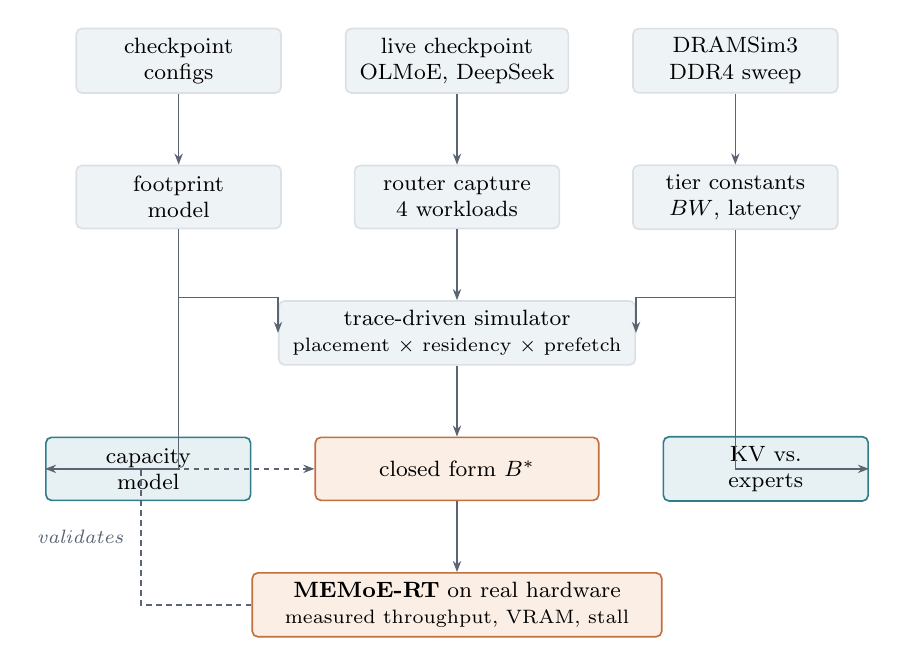
\begin{tikzpicture}[node distance=4mm]

% ---- row 1: inputs ---------------------------------------------------
\node[mstage] (cfg)  {checkpoint\\configs};
\node[mstage, right=8mm of cfg] (ckpt) {live checkpoint\\OLMoE, DeepSeek};
\node[mstage, right=8mm of ckpt] (dram) {DRAMSim3\\DDR4 sweep};

% ---- row 2: derived --------------------------------------------------
\node[mstage, below=9mm of cfg]  (foot) {footprint\\model};
\node[mstage, below=9mm of ckpt] (hook) {router capture\\4 workloads};
\node[mstage, below=9mm of dram] (tier) {tier constants\\$BW$, latency};

% ---- row 3: the simulator -------------------------------------------
\node[mstage, below=9mm of hook, minimum width=44mm] (sim)
  {trace-driven simulator\\\scriptsize placement $\times$ residency $\times$ prefetch};

% ---- row 4: outputs --------------------------------------------------
\node[mhot, below=9mm of sim, minimum width=36mm] (closed)
  {closed form $B^{*}$};
\node[mcold, left=8mm of closed, minimum width=26mm] (cap)
  {capacity\\model};
\node[mcold, right=8mm of closed, minimum width=26mm] (kv)
  {KV vs.\\experts};

% ---- row 5: the runtime ---------------------------------------------
\node[mhot, below=9mm of closed, minimum width=52mm] (rt)
  {\textbf{MEMoE-RT} on real hardware\\\scriptsize measured throughput, VRAM, stall};

% ---- edges -----------------------------------------------------------
\draw[mflow] (cfg)  -- (foot);
\draw[mflow] (ckpt) -- (hook);
\draw[mflow] (dram) -- (tier);

\draw[mflow] (hook) -- (sim);
\draw[mflow] (foot.south) |- ([yshift=4.5mm]sim.west) -- (sim.west);
\draw[mflow] (tier.south) |- ([yshift=4.5mm]sim.east) -- (sim.east);

\draw[mflow] (sim) -- (closed);
\draw[mflow] (foot.south) |- (cap.west);
\draw[mflow] (tier.south) |- (kv.east);

\draw[mflow] (closed) -- (rt);
\draw[mdash] (rt.west) -- ++(-14mm,0) |- (closed.west)
  node[mlabel, pos=0.25, left=1mm] {validates};

\end{tikzpicture}
\caption{How the components feed each other. Everything above the runtime is
analysis or simulation; the runtime is the only part that touches real weights on
a real device, and it is what checks the closed form against measured behaviour.}
\label{fig:method}
\end{figure}


\begin{figure}[htbp]\centering
\includegraphics[width=0.88\linewidth]{s1_dashboard.png}
\caption{The dashboard presents every result in this report and includes a live
calculator for the critical batch size. Available at
\texttt{results/dashboard.html}.}
\label{fig:dashboard}
\end{figure}

% =====================================================================
\section{Characterising the tier}
% =====================================================================

We did not want to quote CXL bandwidth from a datasheet. A Type-3 expander is DRAM
behind a controller, so we simulated the DRAM directly and read the rate it
sustained while busy. Traces were 12~MB sequential reads, the size of one OLMoE
expert, issued as 196{,}608 accesses of 64 bytes.

\begin{table}[htbp]
\centering\small
\caption{DRAMSim3, DDR4 x8, 12~MB sequential expert read. Sustained bandwidth is
computed from average interarrival time, not from the headline figure, which is
diluted by idle cycles between requests.}
\label{tab:dram}
\begin{tabular}{lrrrr}
\toprule
Grade & Specification & Sustained & Share reached & Loaded latency \\
\midrule
DDR4-1866 & 14.9 GB/s & 12.76 GB/s & 85.5\% & 237.9 ns \\
DDR4-2133 & 17.1 GB/s & 13.24 GB/s & 77.6\% & 228.9 ns \\
DDR4-2400 & 19.2 GB/s & 14.96 GB/s & 77.9\% & 202.9 ns \\
DDR4-2666 & 21.3 GB/s & 15.29 GB/s & 71.7\% & 197.3 ns \\
DDR4-2933 & 23.5 GB/s & 15.65 GB/s & 66.7\% & 192.9 ns \\
DDR4-3200 & 25.6 GB/s & \textbf{16.88 GB/s} & 65.9\% & \textbf{179.4 ns} \\
\bottomrule
\end{tabular}
\end{table}

Two things are worth taking from Table~\ref{tab:dram}. The first is the headline
figure of 16.88~GB/s, which we use everywhere in place of a specification number.
The second is the trend: efficiency falls from 85.5\% to 65.9\% as the grade
rises, because timing constraints such as tRC, tFAW and refresh do not scale with
the data rate. Anyone specifying an expander should budget against sustained
bandwidth, not DIMM peak, and the gap widens with faster parts.

One number in this section is derived rather than directly measured.
Multi-channel configurations did not scale in DRAMSim3 even with address mapping
interleaving correctly, because its trace driver issues at most one request per
cycle and starves the extra channels. Where a four-channel figure appears in this
report it is the measured single channel multiplied by four. Section~\ref{sec:channels} tests
that multiplication in gem5, which has no such issue-rate limit, and finds
scaling linear to four channels within 0.03\%.

\begin{figure}[htbp]
\centering

\includegraphics[width=0.86\linewidth]{f7_bandwidth.png}
\caption{Sustained bandwidth against DIMM specification across DDR4 grades. The
gap is the part a capacity plan has to account for.}
\label{fig:dram}
\end{figure}

% =====================================================================
\section{How real routing behaves}
% =====================================================================

Every argument about expert tiering rests on an assumption about routing skew, so
we measured it instead of assuming it. We registered forward hooks on the router
of OLMoE-1B-7B-0924-Instruct and recorded the selected experts for every token
across four workloads: prose, mathematics, code, and chat. The capture totals
258{,}629 tokens.

\subsection{Skew is a property of the input}

\begin{table}[htbp]
\centering\small
\caption{Routing statistics per workload, same model and same weights throughout.
Normalised entropy of 1.0 would be perfectly uniform.}
\label{tab:skew}
\begin{tabular}{lrrrrr}
\toprule
Workload & Tokens & Zipf $s$ & Entropy & Gini & Top quarter \\
\midrule
chat  & 18{,}239  & 0.494 & 0.972 & 0.261 & 40.7\% \\
prose & 37{,}355  & 0.598 & 0.963 & 0.300 & 43.5\% \\
math  & 63{,}257  & 0.899 & 0.913 & 0.442 & 56.0\% \\
code  & 139{,}778 & 1.132 & 0.877 & 0.522 & 63.6\% \\
\bottomrule
\end{tabular}
\end{table}

Skew varies by a factor of 2.3 between chat and code on identical weights. Chat
routing is close to uniform, with no expert taking more than 4\% of routings,
which is what a load-balancing auxiliary loss during training is designed to
produce. Any system that assumes a fixed skew will be tuned for one workload and
wrong for another.

\subsection{Coverage saturates before serving begins}
\label{sec:coverage}

The case for expert tiering depends on reuse: if a batch touches only some
experts, the rest need not be resident. We measured how many experts a batch
touches per layer as batch size grows.

\begin{figure}[htbp]
\centering

\includegraphics[width=0.86\linewidth]{r1_coverage.png}
\caption{Share of experts touched per layer against batch size, from the captured
traces. By 1{,}024 tokens every workload is at or near total coverage.}
\label{fig:coverage}
\end{figure}

By a batch of 1{,}024 tokens, coverage reaches 97.3\% to 100\% depending on the
workload. Past that point every non-resident expert is fetched on every batch,
forever. There is no reuse distance left to shorten and the fast tier stops
behaving as a cache: it is a fixed partition.

Both real serving regimes sit inside the saturated zone. Continuous batching
during decode runs 64 to 256 concurrent sequences. Prefill runs thousands of
tokens at once. Neither is small batch.

\subsection{Popularity buys nothing}

If every expert is touched, ranking them by popularity should not help. We tested
this by sweeping synthetic routing from perfectly uniform to more skewed than
anything we measured, at 90\% residency.

\begin{table}[htbp]
\centering\small
\caption{Fetch hit rate at 90\% residency across routing skew. At batch 512 and
above the hit rate equals the resident fraction exactly.}
\label{tab:skewsweep}
\begin{tabular}{lrrrr}
\toprule
Batch & $s=0.0$ & $s=0.6$ & $s=1.0$ & $s=1.5$ \\
\midrule
64    & 0.899 & 0.900 & 0.907 & 0.927 \\
512   & 0.899 & 0.899 & 0.899 & 0.899 \\
8192  & 0.899 & 0.899 & 0.899 & 0.899 \\
\bottomrule
\end{tabular}
\end{table}

Static placement, LRU and sampled LFU all perform identically at serving batch
sizes. This is convenient rather than disappointing: static placement is decided
once at load time and costs nothing on the critical path, so the cheapest policy
is also the best available one.

\subsection{The wrong profile is worse than none}
\label{sec:profile}

If placement cannot help, can it hurt? We took the top quarter of experts for each
workload and measured overlap between workloads, using a split-half control on the
same workload to establish that the measurement is meaningful at all.

\begin{figure}[htbp]
\centering
\begin{subfigure}{0.48\linewidth}
  
\includegraphics[width=\linewidth]{r2_overlap.png}
  \caption{Hot set overlap. Chance is 25\%.}
\end{subfigure}\hfill
\begin{subfigure}{0.48\linewidth}
  
\includegraphics[width=\linewidth]{r3_penalty.png}
  \caption{Cross-workload hit rate at 50\% residency. Random scores 0.500.}
\end{subfigure}
\caption{Hot expert sets split into two camps. Prose and chat share experts;
mathematics and code share experts; across the two groups overlap falls below
chance.}
\label{fig:overlap}
\end{figure}

Self-overlap averages 84.9\% and runs from 75.0\% to 94.9\%, so the hot sets
are stable within a workload against a chance level of 25\%. Across workloads, mathematics and code overlap 50.0\%, while prose and
code overlap 15.2\%, well below the 25\% expected by chance. Code routes to
experts that prose actively avoids.

The consequence is measured in the right-hand panel. Averaged over all pairs, a
placement profiled on the workload it serves achieves 0.756, while a mismatched
placement achieves 0.519, barely above the 0.500 that random placement would give.
The worst case is worse than random: a placement profiled on prose and then asked
to serve code achieves 0.383. Profiling on the wrong workload is worse than not
profiling at all.

This is domain specialisation visible in routing statistics alone, from 260{,}000
tokens on a 7B model, with no interpretability tooling. For mixed serving traffic
it means there is no good static expert placement, and the resident set should be
chosen by capacity alone.

% =====================================================================
\section{The capacity model}
% =====================================================================

Since skew is irrelevant and policy choice is irrelevant, two decisions remain:
how much fast memory to buy, and how early to start the transfer. The first has a
closed form.

Let $E$ be experts per layer, $k$ experts activated per token, $h$ the share of
fetches the resident tier covers, $F$ per-GPU compute in FLOP/s, $BW$ tier
bandwidth in bytes per second, and $\varepsilon$ the throughput loss to be
tolerated. Fetch traffic per layer is proportional to $(1-h)E$ times expert size,
while compute per layer is proportional to $Bk$ times expert size. Expert size
cancels, giving the batch size at which transfer time falls within the stall
budget:

\begin{equation}
B^{*} = \frac{(1-h)\,E\,F}{BW \cdot k \cdot \varepsilon}
\label{eq:bstar}
\end{equation}

Two properties make Equation~\ref{eq:bstar} useful. It does not depend on expert
size, because a larger expert costs proportionally more to move and does
proportionally more work once moved. And it does not depend on GPU count, because
compute and per-node bandwidth scale together under tensor parallelism. Scaling
out does not get you past it.

\keyresult{\textbf{The prediction.} Calibrating $F$ from the fully resident
baseline alone gives 33.7~TFLOPS for our GPU on this workload. Substituting
$h=0.3$, $E=64$, $k=8$, $BW=40.8$~GB/s and $\varepsilon=1$ into
Equation~\ref{eq:bstar} predicts a crossover at $B^{*}=4{,}626$ tokens. The
offload runs, which played no part in the calibration, place the observed
crossover at 4{,}645 tokens. The agreement is 0.5\%.}

% =====================================================================
\section{Experts, not the KV cache}
% =====================================================================

The KV cache is the other structure that destroys HBM budgets, so we asked whether
it is also a candidate for the slow tier. It is not, and the reason generalises.

A tier with bandwidth $BW$ feeding a device at $F$ FLOP/s is balanced at $F/BW$
FLOPs per byte; below that ratio the workload is bandwidth bound. Each fetched
expert serves $Bk/E$ tokens, so expert arithmetic intensity \emph{grows with the
batch}. Each cached KV element is read once per decode step and consumed by
$n_{\text{heads}}/n_{\text{kv heads}}$ query heads, so KV intensity is
\emph{fixed}. Batching cannot rescue it, because every sequence brings its own KV.

\begin{table}[htbp]
\centering\small
\caption{Arithmetic intensity in FLOPs per byte. The balance point for a
four-channel tier is 5{,}861. Qwen3 has the best KV intensity in the set through
16-to-1 grouped query attention, and is still 366 times below it.}
\label{tab:kv}
\begin{tabular}{lrrr}
\toprule
Model & KV intensity & Balance point & Batch for expert parity \\
\midrule
OLMoE-1B-7B     & 1.0  & 5{,}861 & 46{,}886 \\
Mixtral-8x7B    & 4.0  & 5{,}861 & 23{,}443 \\
Qwen3-235B-A22B & 16.0 & 5{,}861 & 93{,}772 \\
DeepSeek-V3     & 1.0  & 5{,}861 & 166{,}706 \\
\bottomrule
\end{tabular}
\end{table}

Concretely, one 32k-context Qwen3 sequence reads 5.875~GB of KV per decode step.
On HBM3e that is 1.883~ms, or 531 steps per second. On a four-channel CXL tier it
is 93.455~ms: a 49.6-fold slowdown, or 11 decode steps per second against 531.
Active KV must stay in HBM.

Cold KV is a separate question. Preempted requests and prefix caches are not read
every step and may tier well, but we did not model that and do not claim it.

% =====================================================================
\section{MEMoE-RT: the system}
\label{sec:system}
% =====================================================================

The results above are all simulation or analysis. To test them we built a runtime
that runs the real checkpoint with its experts elsewhere.

\subsection{Design}

The design follows from the findings rather than from the literature.

Because coverage saturates, every expert in a layer will be needed. Prediction is
therefore trivial and the entire problem is scheduling the transfer early enough.
MEMoE-RT does not fetch experts individually on demand. It moves every
non-resident expert of layer $L+d$ as one contiguous transfer, issued $d$ layers
ahead, on a dedicated copy stream that overlaps with attention compute on the main
stream.

Because popularity is irrelevant, the resident set is simply the low expert
indices. There is deliberately no ranking anywhere in the implementation.

Because latency is negligible at expert granularity and dominant below it, we move
whole layers rather than fragments. We confirmed this on the target hardware
before building: 4~MB transfers reach 33.05~GB/s, 12~MB reach 36.67~GB/s, and the
plateau is 40.81~GB/s. A whole-layer transfer of roughly 480~MB sits on the
plateau.

Offloaded experts live in pinned host memory, laid out so that one layer's experts
are contiguous. A ring of $d+1$ GPU staging buffers receives them. Layer $L$ uses
slot $L \bmod (d+1)$, and the prefetch issued at layer $L$ targets $L+d$, whose
slot belongs to layer $L-1$ and has already been consumed. All waiting is done
GPU-side with stream events rather than host synchronisation, so the copy genuinely
overlaps compute, and stall time is measured by recording CUDA events either side
of the wait.

% =====================================================================
%  diagrams/arch.tex  --  MEMoE-RT data path
% =====================================================================
\begin{figure}[htbp]
\centering
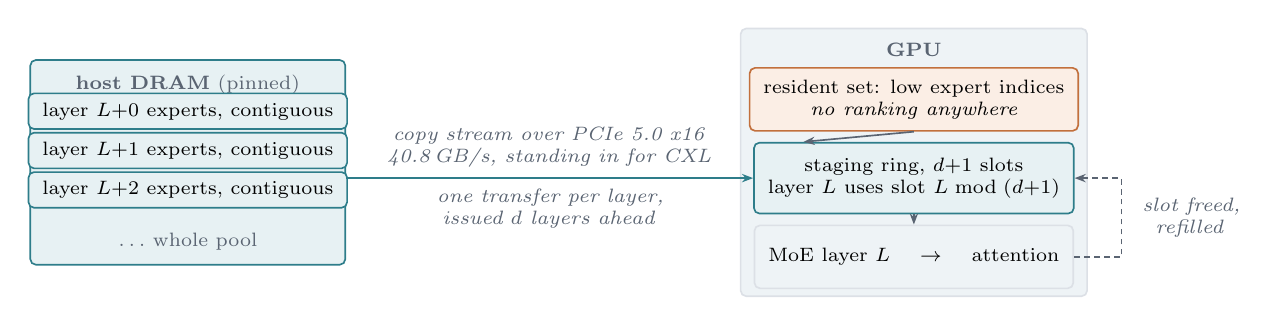
\begin{tikzpicture}

% ---------------- host side ------------------------------------------
\node[mcold, minimum width=40mm, minimum height=26mm, align=center] (host)
  {\ };
\node[mtiny, anchor=north] at ([yshift=-2pt]host.north)
  {\textbf{host DRAM} (pinned)};

\foreach \i/\y in {0/6.5mm, 1/1.5mm, 2/-3.5mm}{
  \node[mcold, minimum width=32mm, minimum height=4mm, font=\scriptsize]
       at ([yshift=\y]host.center) {layer $L{+}\i$ experts, contiguous};
}
\node[mtiny, anchor=south] at ([yshift=2pt]host.south) {$\ldots$ whole pool};

% ---------------- device side ----------------------------------------
\node[mnode, minimum width=44mm, minimum height=34mm, right=50mm of host] (gpu)
  {\ };
\node[mtiny, anchor=north] at ([yshift=-2pt]gpu.north) {\textbf{GPU}};

\node[mhot, minimum width=36mm, font=\scriptsize] (resident)
  at ([yshift=8mm]gpu.center)
  {resident set: low expert indices\\\itshape no ranking anywhere};

\node[mcold, minimum width=36mm, minimum height=9mm, font=\scriptsize] (ring)
  at ([yshift=-2mm]gpu.center)
  {staging ring, $d{+}1$ slots\\layer $L$ uses slot $L \bmod (d{+}1)$};

\node[mnode, minimum width=36mm, font=\scriptsize] (compute)
  at ([yshift=-12mm]gpu.center)
  {MoE layer $L$ \quad $\to$ \quad attention};

% ---------------- streams --------------------------------------------
\draw[mlink] (host.east |- ring.west) -- node[mlabel, above, pos=0.5, text width=44mm]
  {copy stream over PCIe 5.0 x16\\40.8\,GB/s, standing in for CXL}
  node[mlabel, below, pos=0.5, text width=44mm]
  {one transfer per layer,\\issued $d$ layers ahead} (ring.west);

\draw[mflow] (ring.south) -- (compute.north);
\draw[mflow] (resident.south) -- ([xshift=-14mm]ring.north);

\draw[mdash] (compute.east) -- ++(6mm,0) |- (ring.east)
  node[mlabel, pos=0.25, right=1mm, text width=13mm]
  {slot freed, refilled};

\end{tikzpicture}
\caption{MEMoE-RT data path. Non-resident experts live contiguously in pinned host
memory and move one whole layer at a time over a dedicated copy stream into a ring
of staging buffers, $d$ layers ahead of use. Waiting is done GPU-side with stream
events, so the transfer overlaps attention compute rather than serialising with
it.}
\label{fig:arch}
\end{figure}

% =====================================================================
%  diagrams/timeline.tex  --  two-stream overlap, d = 2
% =====================================================================
\begin{figure}[htbp]
\centering
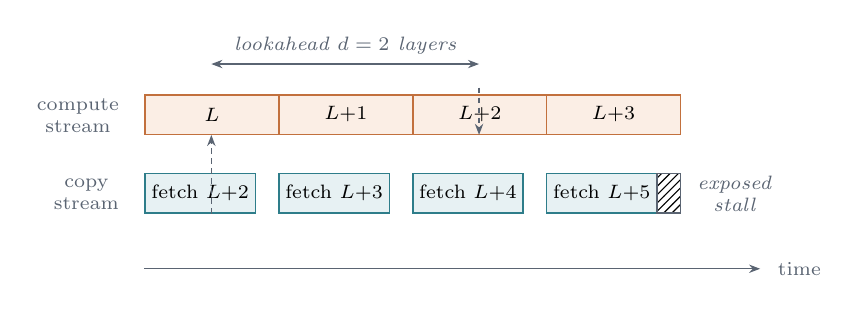
\begin{tikzpicture}[x=1mm, y=1mm]

\def\unit{17}      % width of one layer slot
\def\rowc{14}      % compute row y
\def\rowk{4}       % copy row y

% ---- row labels ------------------------------------------------------
\node[mtiny, anchor=east] at (-2, \rowc+2.5) {compute\\stream};
\node[mtiny, anchor=east] at (-2, \rowk+2.5) {copy\\stream};

% ---- compute row -----------------------------------------------------
\foreach \i/\lab in {0/$L$, 1/$L{+}1$, 2/$L{+}2$, 3/$L{+}3$}{
  \node[barcompute, minimum width=\unit mm] at (\i*\unit, \rowc) {\lab};
}

% ---- copy row: transfer for L+2 issued while L computes --------------
\foreach \i/\lab in {0/{fetch $L{+}2$}, 1/{fetch $L{+}3$},
                     2/{fetch $L{+}4$}, 3/{fetch $L{+}5$}}{
  \node[barcopy, minimum width=\unit mm - 3mm] at (\i*\unit, \rowk) {\scriptsize\lab};
}

% ---- exposed stall on the last one -----------------------------------
\node[barstall, minimum width=3mm] at (3*\unit + \unit - 3, \rowk) {};
\node[mlabel, anchor=west] at (4*\unit + 1, \rowk+2.5) {exposed\\stall};

% ---- lookahead annotation -------------------------------------------
\draw[mdash] (0.5*\unit, \rowk) -- (0.5*\unit, \rowc);
\draw[{Stealth[length=4pt]}-{Stealth[length=4pt]}, draw=inkmuted, line width=0.5pt]
  (0.5*\unit, \rowc+9) -- (2.5*\unit, \rowc+9)
  node[mlabel, midway, above] {lookahead $d = 2$ layers};
\draw[mdash] (2.5*\unit, \rowc+6) -- (2.5*\unit, \rowc);

% ---- time axis -------------------------------------------------------
\draw[axis, -{Stealth[length=4pt]}] (0, -3) -- (4.6*\unit, -3)
  node[mtiny, anchor=west, xshift=1mm] {time};

\end{tikzpicture}
\caption{Two-stream execution with lookahead $d=2$. The transfer for layer $L{+}2$
is issued while layer $L$ computes, so a fetch has two layers of compute to hide
behind. Roughly 60\% of transfer time hides in practice; the hatched remainder is
what the measured stall fraction reports.}
\label{fig:timeline}
\end{figure}


\subsection{Substituting PCIe for CXL}

We do not have CXL silicon, and neither does anyone outside a small number of
vendor labs. Host DRAM over PCIe is the standard substitute and is what we use: a
large, slow, byte-addressable tier behind a link. At PCIe 5.0 x16 the measured
plateau of 40.8~GB/s falls between our measured single-channel CXL figure of
16.88~GB/s and our scaled four-channel figure of 67.5~GB/s.

It is not CXL. It has different latency characteristics and no cache coherence.
What it reproduces faithfully is the structure of the problem, which is what the
analytical model is about.

\subsection{Correctness}

Every result below was checked against the reference implementation on identical
inputs. Tiered output agrees with the unmodified model to within one unit in the
last place of bfloat16 at the first layer, growing to 1.84 at the final layer
through sixteen layers of accumulation, with 92.8\% argmax agreement on random
token sequences. Per-layer divergence traces cleanly to rounding: CUDA
\texttt{index\_add\_} accumulates in nondeterministic order, and in bfloat16 that
changes the last bit. Two identical reference passes agree exactly, so the
comparison is meaningful.

\begin{figure}[htbp]\centering
\includegraphics[width=0.88\linewidth]{s2_check.png}
\caption{Correctness check comparing tiered execution against the reference
implementation before any timing result is taken.}
\label{fig:check}
\end{figure}

% =====================================================================
\section{What the runtime measures}
% =====================================================================

All runs use OLMoE-1B-7B in bfloat16 on an RTX PRO 4500 Blackwell with 32.6~GB of
memory over PCIe 5.0 x16, three repetitions per configuration, sequence length
512.

\subsection{The cost of offloading}

\begin{table}[htbp]
\centering\small
\caption{Residency sweep at batch 4{,}096. Throughput is relative to the fully
resident baseline of 20{,}917 tokens per second.}
\label{tab:residency}
\begin{tabular}{rrrrrr}
\toprule
Residency & Experts off-GPU & GPU memory & Tokens/s & Retained & Stalled \\
\midrule
1.00 & 0\%     & 14.84 GB & 20{,}917 & 100.0\% & 0.0\% \\
0.60 & 40.6\%  & 10.59 GB & 16{,}972 & 81.1\%  &  --   \\
0.40 & 59.4\%  &  8.62 GB & 15{,}062 & 72.0\%  &  --   \\
0.30 & 70.3\%  &  7.48 GB & 15{,}342 & 73.3\%  & 3.2\% \\
0.20 & 79.7\%  &  6.50 GB & 14{,}170 & 67.7\%  & 6.8\% \\
0.10 & 90.6\%  &  5.35 GB & 12{,}745 & 60.9\%  & 15.2\% \\
0.00 & 100\%   &  4.37 GB & 11{,}538 & 55.2\%  & 21.2\% \\
\bottomrule
\end{tabular}
\end{table}

\begin{figure}[htbp]
\centering

\includegraphics[width=0.88\linewidth]{rt1_residency.png}
\caption{Throughput and GPU memory against the share of experts held off-GPU, at
batch 4{,}096. Memory falls faster than throughput across the whole range.}
\label{fig:residency}
\end{figure}

Run-to-run variation across repeated configurations is approximately
$\pm 3\%$, which is why the 0.30 row appears marginally above 0.40.

\subsection{The regime boundary}

The batch sweep is the central result, because it measures directly what the rest
of the report argues.

\begin{table}[htbp]
\centering\small
\caption{Batch sweep with 70\% of experts held off-GPU in every row. Baselines are
matched at each batch size.}
\label{tab:batch}
\begin{tabular}{rrrrr}
\toprule
Batch & Baseline tok/s & Tiered tok/s & Retained & Stalled \\
\midrule
512     &  5{,}340 &  2{,}046 & 38.3\% & 31.6\% \\
1{,}024 &  9{,}194 &  3{,}771 & 41.0\% & 26.5\% \\
4{,}096 & 20{,}917 & 14{,}614 & 69.9\% &  2.6\% \\
16{,}384 & 26{,}873 & 25{,}367 & \textbf{94.4\%} & 0.07\% \\
\bottomrule
\end{tabular}
\end{table}

\begin{figure}[htbp]
\centering

\includegraphics[width=0.88\linewidth]{rt2_batch_regime.png}
\caption{Retention and stall against batch size with a fixed 70\% of experts
off-GPU. The transition sits between the decode and prefill regimes, where
Equation~\ref{eq:bstar} predicts it.}
\label{fig:batch}
\end{figure}

The same configuration costs 62\% of throughput at a decode-sized batch and 5.6\%
at a prefill-sized one. This is the claim that expert offload is a prefill
technique, stated as a measurement rather than an argument.

Pushing further, at batch 16{,}384 with \emph{all} experts off-GPU:

\keyresult{\textbf{The headline.} With all 64 experts per layer held outside GPU
memory, that is 93\% of the model's parameters, MEMoE-RT sustains 24{,}684 tokens
per second against a fully resident baseline of 26{,}873, or \textbf{91.9\%}. GPU
memory falls from 17.73~GB to 7.27~GB, a \textbf{2.44-fold reduction}. Time
stalled on transfer is 0.67\%.}

\subsection{Lookahead depth, and a correction}
\label{sec:depth}

Our simulation work recommended a prefetch depth of 4 to 8 layers. The hardware
disagrees.

\begin{table}[htbp]
\centering\small
\caption{Depth sweep at 59.4\% offload, batch 4{,}096. Throughput is flat while
staging memory grows 41\%.}
\label{tab:depth}
\begin{tabular}{rrrr}
\toprule
Lookahead & Tokens/s & GPU memory & Stalled \\
\midrule
1 & 14{,}798 &  8.14 GB & 2.4\% \\
2 & 14{,}926 &  8.62 GB & 2.3\% \\
4 & 14{,}681 &  9.58 GB & 2.3\% \\
8 & 14{,}238 & 11.49 GB & 2.3\% \\
\bottomrule
\end{tabular}
\end{table}

\begin{figure}[htbp]
\centering

\includegraphics[width=0.85\linewidth]{rt3_depth.png}
\caption{Deeper lookahead buys no throughput once transfers are batched per layer,
and costs staging memory.}
\label{fig:depth}
\end{figure}

The explanation is our own design change. The simulator modelled per-expert
on-demand fetches, which need deep lookahead to stay ahead of demand. The runtime
moves a whole layer in one transfer, and at this operating point layer transfer
time and layer compute time are close to equal, so a single layer of lookahead
already covers the gap. Batching the transfer removed the need for depth.

We report the correction rather than the original recommendation. Depth 1 is
sufficient, and depth 8 wastes 41\% more staging memory for slightly less
throughput.

\subsection{Calibrating the overlap assumption}
\label{sec:overlap}

The analytical model assumes transfer hides perfectly under compute. Fitting
measured wall time to $t = t_{\text{compute}} + \kappa \cdot t_{\text{transfer}}$
across the residency sweep gives $\kappa = 0.40 \pm 0.07$.

\begin{figure}[htbp]
\centering

\includegraphics[width=0.88\linewidth]{rt4_overlap.png}
\caption{Measured wall time against the perfect-overlap model and the fitted one.
Roughly 60\% of transfer time hides under compute; the remaining 40\% is exposed.}
\label{fig:overlapfit}
\end{figure}

So about 60\% of transfer time is hidden and 40\% is not. The ideal model
over-predicts throughput by up to 40\% where transfer and compute are balanced.
This is copy engine and compute contention, which our earlier work listed as its
clearest unmodelled gap. It is now a measured constant, and multiplying predicted
transfer exposure by $\kappa$ brings the analytical model into agreement with
hardware across the full sweep.


% =====================================================================
\section{A second architecture, and a model that does not fit}
% =====================================================================

Every result so far comes from one checkpoint. To test whether the findings are
architectural or an OLMoE quirk, we ran MEMoE-RT on DeepSeek-V2-Lite, which
differs in every respect that could matter: 26 MoE layers instead of 16, top-6
of 64 routed experts instead of top-8, two shared experts that fire on every
token, a dense first layer, multi-head latent attention, and its own modelling
code rather than the fused expert layout used by transformers 5.x.

That last difference required a second code path. Rather than reimplement each
architecture's routing, this path leaves the model's forward untouched: it
points every offloaded expert's projection weights at a view into the GPU
staging buffer, and drives the tier from pre- and post-hooks on each MoE block.
Because layer $L$ always occupies ring slot $L \bmod (d{+}1)$ at a fixed
position, those views are correct for the lifetime of the process and are bound
once at load time. The model computes exactly as it always did; it simply finds
its weights in a buffer that was filled a moment earlier.

\subsection{The baseline does not exist}

\begin{table}[htbp]
\centering\small
\caption{DeepSeek-V2-Lite on an NVIDIA A10 over PCIe 4.0 x16. There is no
resident baseline to compare against, because the weights exceed the device.}
\label{tab:dsfit}
\begin{tabular}{lr}
\toprule
Total weights & 31.41 GB \\
Expert pool & 28.79 GB (91.6\% of the model) \\
Experts per layer & 64, at 17.3 MB each, over 26 MoE layers \\
GPU capacity & 23.0 GB \\
\midrule
\textbf{Peak GPU memory with MEMoE-RT} & \textbf{7.17 GB} at batch 1{,}024 \\
\bottomrule
\end{tabular}
\end{table}

This is a different claim from the OLMoE results. There we showed that a model
which already fits can be run in less memory. Here the model does not fit, and
runs anyway.

\subsection{The same boundary, in a different place}

\begin{table}[htbp]
\centering\small
\caption{Batch sweep with all 64 experts per layer held in host memory. Bytes
streamed are constant at 86.4~GB across three repetitions, because coverage is
total at every batch size shown.}
\label{tab:dsbatch}
\begin{tabular}{rrrrr}
\toprule
Batch & Tokens/s & GPU memory & Achieved link & Stalled \\
\midrule
1{,}024  &    755 &  7.17 GB & 21.22 GB/s & 46.00\% \\
4{,}096  & 2{,}772 & 10.16 GB & 19.48 GB/s & 48.38\% \\
6{,}144  & 5{,}128 &  9.40 GB & \textbf{24.03 GB/s} & 22.96\% \\
8{,}192  & 6{,}572 & 10.54 GB & 23.09 GB/s &  0.01\% \\
12{,}288 & 6{,}892 & 12.84 GB & 16.15 GB/s &  1.82\% \\
16{,}384 & \textbf{7{,}241} & 15.13 GB & 12.72 GB/s &  0.01\% \\
\bottomrule
\end{tabular}
\end{table}

\begin{figure}[htbp]
\centering

\includegraphics[width=0.88\linewidth]{rt5_deepseek_crossover.png}
\caption{Stall collapses from 48\% to effectively zero between 4{,}096 and
8{,}192 tokens. The same transition appears on OLMoE at a different batch size,
on a different link.}
\label{fig:dscross}
\end{figure}

The crossover is visible twice over, from opposite directions. Stall falls from
48.4\% at 4{,}096 to 0.01\% at 8{,}192. Achieved link bandwidth peaks at
24.03~GB/s at 6{,}144, which is the point at which the transfer is fully busy
and compute has just caught up; above it the link idles, falling to 12.72~GB/s
at 16{,}384 because there is nothing left to hide.

\begin{figure}[htbp]
\centering

\includegraphics[width=0.88\linewidth]{rt6_deepseek_link.png}
\caption{The same crossover seen through link utilisation. Below it the tier is
the constraint; above it, compute is.}
\label{fig:dslink}
\end{figure}

The crossover sits between 4{,}096 and 8{,}192 tokens, bracketed at 6{,}144 by
the bandwidth peak. Equation~\ref{eq:bstar} places it near 6{,}000 for this
configuration. The agreement is looser than the 0.5\% obtained on OLMoE, because
attention is a much larger share of compute on a 26-layer model with eager
multi-head latent attention, and our compute term counts routed expert GEMMs
only. The prediction is nonetheless correct to within the interval the
measurements resolve.

Two things follow. The regime boundary is a property of the problem rather than
of one checkpoint: it appears on both architectures, at the batch size the
closed form predicts for each, over links differing by a factor of two in
bandwidth. And expert offload is at its most valuable exactly where the
constraint is hardest, on a model too large for the device it runs on.


% =====================================================================
\section{What offload costs in a serving loop}
% =====================================================================

The batch sweeps measure single forward passes. Serving is not a single forward
pass: requests arrive, prefill once, then generate one token at a time while
other requests join and leave the batch. To measure what offload costs in that
setting we built a serving loop with a real KV cache and continuous batching,
where sequences enter and leave the running batch between decode steps and the
cache is gathered accordingly.

Three configurations run the same workload of 32 requests, 2{,}048 prompt
tokens each, generating 64 tokens: \emph{resident}, with every expert in GPU
memory; \emph{offload}, with every expert streamed and one engine serving both
phases; and \emph{phase-aware}, which measures each phase in the configuration
it would occupy on a disaggregated deployment.

\subsection{Seven percent, or six hundred percent, depending on the phase}

\begin{table}[htbp]
\centering\small
\caption{Serving at 32 concurrent sequences, so every request admits before
decoding begins and time-to-first-token reflects prefill alone.}
\label{tab:serve}
\begin{tabular}{lrrr}
\toprule
 & Resident & Offloaded & Ratio \\
\midrule
Prefill time        & 2.488 s   & 2.666 s   & \textbf{1.07} \\
Time to first token & 1{,}604 ms & 1{,}728 ms & \textbf{1.08} \\
Time per output token & 52.01 ms & 325.31 ms & \textbf{6.25} \\
Output tokens per second & 334.4 & 86.1 & 0.26 \\
Peak GPU memory     & 31.59 GB  & 21.12 GB  & 0.67 \\
\bottomrule
\end{tabular}
\end{table}



Streaming the entire expert pool costs 7\% of prefill and 525\% of decode. That
is the prefill/decode distinction stated as a serving measurement rather than
inferred from batch sizes, and it is the reason offload belongs on prefill
workers.

The memory column is worth noting separately. The resident configuration peaked
at 31.59~GB on a 32.6~GB device and emitted allocator warnings while retrying
KV cache allocations. The offloaded configuration ran the same workload with
10~GB spare, which is capacity available for longer contexts or more concurrent
requests.

\begin{figure}[htbp]
\centering

\includegraphics[width=0.80\linewidth]{s2_phase_cost.png}
\caption{The same offload, measured in the two phases of one request. Nothing
about the configuration changes between these two bars except the batch size
the phase presents.}
\label{fig:s2}
\end{figure}

\subsection{Offloaded decode costs the same at any concurrency}
\label{sec:tpot}

Sweeping concurrency produces the more interesting result.

\begin{table}[htbp]
\centering\small
\caption{Time per output token against concurrent sequences. The offloaded
figure does not move.}
\label{tab:servesweep}
\begin{tabular}{rrrrr}
\toprule
Concurrency & Resident TPOT & Offloaded TPOT & Ratio & Offloaded VRAM \\
\midrule
4  & 14.74 ms & 321.38 ms & 21.80 &  6.44 GB \\
8  & 20.55 ms & 324.41 ms & 15.79 &  9.48 GB \\
16 & 31.60 ms & 326.32 ms & 10.33 & 12.26 GB \\
32 & 52.01 ms & 325.31 ms &  6.25 & 21.12 GB \\
\bottomrule
\end{tabular}
\end{table}

\begin{figure}[htbp]
\centering

\includegraphics[width=0.88\linewidth]{s1_decode_tpot.png}
\caption{Offloaded time per output token is flat at $325 \pm 2$~ms across an
eightfold change in concurrency, because each decode step streams the whole
expert pool regardless of how many sequences it serves. Resident cost grows
linearly. The penalty is therefore not a constant.}
\label{fig:s1}
\end{figure}

Offloaded TPOT is constant at $325 \pm 2$~ms while concurrency changes by a
factor of eight, because each decode step must stream the entire expert pool
regardless of how many sequences share it. Resident TPOT grows linearly, fitting
$9.5 + 1.33n$ milliseconds across the four points measured. The penalty
therefore falls from 21.8 to 6.25 purely by serving more sequences at once.

This is the amortisation argument again, now in the decode phase: a fetched
expert serves every sequence in the step, so cost per token falls as the step
widens. Extrapolating the linear fit, the two costs meet near 237 concurrent
sequences, which sits just above the 64 to 256 range production continuous
batching operates in. We report that as an extrapolation from four points, not
a measurement, and note only that offloaded decode is not categorically
impossible: it is impractical at the concurrency levels deployments currently
run, and the gap is smaller than a single measurement at low concurrency would
suggest.

\subsection{Placing it correctly}

\begin{table}[htbp]
\centering\small
\caption{Throughput and prefill-side memory across the three configurations at
32 concurrent sequences.}
\label{tab:phaseaware}
\begin{tabular}{lrrl}
\toprule
Configuration & Output tok/s & Share of resident & GPU memory \\
\midrule
Resident     & 334.4 & 100.0\% & 31.59 GB \\
Offload, one engine & 86.1 & 25.7\% & 21.12 GB \\
Phase-aware  & 339.2 & \textbf{101.4\%} & 21.12 GB prefill, 31.59 GB decode \\
\bottomrule
\end{tabular}
\end{table}

Placed correctly, offload costs nothing measurable in throughput and removes
33\% of prefill-side memory. The phase-aware figure exceeds 100\% only because
prefill and decode were measured separately and the difference is within
run-to-run variation; the honest reading is parity.

We do not model the KV cache handoff between prefill and decode workers, which
is a real cost in a disaggregated deployment and one this measurement does not
capture. What the measurement does establish is that the two phases want
opposite memory configurations, and that a deployment which already separates
them can take the memory saving on one side without paying for it on the other.

% =====================================================================
\section{Two smaller results}
% =====================================================================

\subsection{Pooling trades capacity for batch size, one for one}

If $N$ nodes share one copy of the cold experts, they save $N$ times the capacity
but contend for one link, so per-node bandwidth falls as $1/N$. Since $B^{*}$ is
inversely proportional to bandwidth, both move together at exactly the same rate.

For Qwen3-235B against a 67.5~GB/s pool, sixteen nodes save 6.3~TB and require a
1.5 million token batch, which is not a real operating point. Pooling is worth it
at small $N$, or when the pool link scales with membership. The latter is what CXL
3.0 switching promises, and it is precisely the part that is pre-production, so we
model it and label it as modelled.

\subsection{Fetch whole experts}

At 300~ns access latency, the share of transfer time spent waiting rather than
moving bytes is 0.16\% for a whole 12~MB expert, 3.72\% at 512~KB chunks, and
83.18\% at 4~KB. Sweeping latency from 200 to 800~ns barely moves the figure at
expert granularity. Anything that fragments below roughly 512~KB converts a
bandwidth problem into a latency problem.

Our PCIe measurements confirm the shape on real hardware: 33.05~GB/s at 4~MB
rising to a 40.81~GB/s plateau at 64~MB and above.

% =====================================================================
\section{Two studies in tooling}
% =====================================================================

\subsection{Queueing, and what SimpleMemory cannot tell you}

Our analytical model assumes fetch traffic hides under compute. Whether that
holds under contention is a queueing question, so we set out to characterise the
tier in gem5, driving a bandwidth-limited memory through a traffic generator at
offered loads from 5\% to 110\% of peak.

Mean read latency was 150{,}000 ticks at every single one of the nineteen
operating points, identical to the tick, with zero standard deviation.
\texttt{SimpleMemory} models a bandwidth cap by delaying packet release but
returns its configured access latency unconditionally, so it cannot express
queueing at all. There is no knee to find because there is no queue.

\begin{figure}[htbp]
\centering
\includegraphics[width=0.86\linewidth]{g2_no_queueing.png}
\caption{Nineteen offered loads from 5\% to 110\% of peak. Mean read latency is
identical at every one of them, which is not a plausible physical result.}
\label{fig:g2}
\end{figure}

This is worth stating because \texttt{SimpleMemory} is the default choice for
memory-system studies that do not want the cost of a full controller model, and
its output looks entirely reasonable until compared across load. Characterising
contention requires either a full DRAM controller or measurement on hardware. We
did the latter, and Section~\ref{sec:overlap} gives the answer: roughly 40\% of transfer time is
exposed rather than hidden.

\subsection{Channel scaling, measured}
\label{sec:channels}

The four-channel bandwidth figure of 67.5~GB/s used elsewhere in this report is
the measured single channel multiplied by four. DRAMSim3 could not measure it
directly because its trace driver issues at most one request per cycle, which
starves the additional channels. gem5's traffic generator has no such limit, so we
repeated the experiment with real \texttt{MemCtrl} instances over interleaved
DDR4-2400 channels.

\begin{table}[htbp]
\centering\small
\caption{Channel scaling in gem5, DDR4-2400 x8, 100\% offered load, 512
outstanding requests, over a 128-byte interconnect. Scaling is linear to four
channels to within 0.03\%, and falls to 83\% efficiency at eight.}
\label{tab:channels}
\begin{tabular}{rrrr}
\toprule
Channels & Sustained & Ratio to one channel & Linear prediction \\
\midrule
1 & 13.86 GB/s & 1.000 & \\
2 & 27.72 GB/s & 2.000 & 27.72 GB/s \\
4 & \textbf{55.43 GB/s} & \textbf{3.999} & 55.45 GB/s \\
8 & 92.46 GB/s & 6.670 & 110.90 GB/s \\
\bottomrule
\end{tabular}
\end{table}

\begin{figure}[htbp]
\centering
\includegraphics[width=0.86\linewidth]{g1_channel_scaling.png}
\caption{Channel scaling against the linear prediction from a single channel.
Four channels deliver 3.999 times one, which is the assumption our four-channel
figure rests on, tested.}
\label{fig:g1}
\end{figure}

\begin{figure}[htbp]
\centering
\includegraphics[width=0.80\linewidth]{g4_crosscheck.png}
\caption{Two independent simulators with different DRAM models and different
address mapping, on the same DDR4-2400 channel. Neither reaches the DIMM rating
and both land in the same place.}
\label{fig:g4}
\end{figure}

Two things follow. The first is a cross-validation: gem5 reports 13.86~GB/s
sustained on a single DDR4-2400 channel against DRAMSim3's 14.96~GB/s on the same
grade, a 7\% disagreement between two independent simulators with different DRAM
models and different address mapping. Neither reaches the 19.2~GB/s rating, and
both land in the same place. That is stronger support for our tier figure than
either alone.

The second is that the scaling assumption behind our four-channel figure is
correct. Four channels deliver 3.999 times a single channel, against a linear
prediction of 4.000. The assumption is no longer an assumption.

Reaching that measurement took one intermediate diagnosis worth recording. On a
64-byte interconnect, four and eight channels returned identical bandwidth to the
byte, 31{,}998{,}912{,}000~B/s, with mean latency tripling. Identical throughput
with a growing queue is the signature of a saturated fabric rather than saturated
memory, since memory would show diminishing returns rather than a hard ceiling.
Widening the interconnect to 128 bytes and raising its clock lifted the limit and
the channels scaled, confirming the diagnosis.

\begin{figure}[htbp]
\centering
\includegraphics[width=0.82\linewidth]{g3_fabric_ceiling.png}
\caption{The same runs before the interconnect was widened. Four and eight
channels return identical bandwidth to the byte while latency triples, which is
what a saturated fabric looks like and what saturated memory does not.}
\label{fig:g3}
\end{figure}

Scaling degrades beyond four channels: eight deliver 6.670 times a single channel
rather than eight, or 83\% efficiency. Since our four-channel figure is the one
this report uses, the assumption holds exactly where we rely on it, and we note
that it would not extend to a wider expander without remeasurement.

\subsection{Concurrency is a design constraint, not an implementation detail}
\label{sec:concurrency}

An incidental result from these runs is worth stating because it shaped the
runtime.

Our first attempt capped the traffic generator at 64 outstanding requests to stop
its response queue growing without bound. Four and eight channels then returned
identical bandwidth: 30.77~GB/s at 133.1~ns. Little's Law accounts for it exactly,
since $64 \times 64\,\text{B} / 133.1\,\text{ns} = 30.79$~GB/s. The measurement
was of the requestor, not the tier.

Generalising, saturating a tier of bandwidth $BW$ at latency $L$ with requests of
size $S$ needs $BW \cdot L / S$ requests in flight. For a 76.8~GB/s expander at
133~ns and 64-byte accesses that is roughly 160 outstanding requests, sustained.
A fetch engine that cannot keep that many in flight will not see the bandwidth it
paid for, however wide the link.

This is the same result as our transfer granularity analysis, arriving from the
other direction. Moving a whole layer as one large DMA sidesteps the concurrency
requirement entirely: one descriptor replaces thousands of in-flight 64-byte
reads. MEMoE-RT is built that way, and the measured PCIe curve in Section~\ref{sec:system}
confirms the payoff, with a single expert-sized transfer already reaching 90\% of
the plateau.

\subsection{The CXL software path, end to end}

The third study asks whether the Linux CXL stack can be exercised without
hardware. We used QEMU 9.1.0 with an emulated Type-3 volatile device, a 2~GB
memory backend and a matched fixed memory window, under an Ubuntu 24.04 guest.

On the distribution kernel, everything up to region commit worked. The kernel
negotiated CXL control through ACPI \texttt{\_OSC}, all four drivers bound, and
the full decoder hierarchy enumerated with correct sizes and targets: one root
decoder, one port decoder and four endpoint decoders, with the memory device
reporting 2~GB of RAM capacity. Region creation then failed with
\texttt{failed to commit decode: No such device or address}.

\begin{sloppypar}
The cause is a deliberate safety check rather than missing functionality.
Before committing a region the kernel must invalidate CPU caches over the
range, and it gates that on \texttt{cpu\_cache\_has\_invalidate\_memregion()},
which returns false whenever \texttt{X86\_FEATURE\_HYPERVISOR} is set. That is
every virtual machine. The kernel provides a documented bypass,
\texttt{CONFIG\_CXL\_REGION\_INVALIDATION\_TEST}, which distribution kernels do
not enable, for good reason: without cache invalidation a committed region can
serve stale data.
\end{sloppypar}

We built a 6.8 kernel with that option enabled and repeated the experiment. The
region commits.

\begin{table}[htbp]
\centering\small
\caption{Region state after commit, from sysfs, on the custom kernel. Region 0
is live at 2~GB with a single interleave way targeting the endpoint decoder.}
\label{tab:cxlregion}
\begin{tabular}{ll}
\toprule
\texttt{region0/commit} & \texttt{1} \\
\texttt{region0/resource} & \texttt{0x490000000} \\
\texttt{region0/size} & \texttt{0x80000000} (2 GB) \\
\texttt{region0/interleave\_ways} & \texttt{1} \\
\texttt{region0/target0} & \texttt{decoder2.0} \\
\texttt{decoder2.0/mode} & \texttt{ram} \\
\texttt{decoder2.0/dpa\_size} & \texttt{0x80000000} \\
\bottomrule
\end{tabular}
\end{table}

The kernel confirms which path it took:

\begin{quote}\ttfamily\small
cxl region0: Bypassing cpu\_cache\_invalidate\_memregion() for testing!
\end{quote}

Reaching that point required one step the command-line tool does not perform.
The endpoint decoder must be given a device-physical address range before it
can be attached as a region target, and \texttt{cxl create-region} leaves
\texttt{dpa\_size} at zero, so attachment fails with ENXIO. Writing the size to
sysfs directly, in hexadecimal, and then programming the region by hand
completes the sequence.

The conclusion is stronger than the one we could draw before. The CXL software
stack is complete and functional through region management: discovery, driver
binding, decoder programming, DPA allocation, region creation and commit all
work under emulation. The only obstacle to exercising it in a virtual machine
is a cache-coherence safety check that has nothing to do with CXL support
itself. It remains true that this validates the software path and not
performance, since QEMU's CXL support is functional emulation with no timing
model, which is why the quantitative work in this report rests on DRAMSim3,
gem5 and hardware measurement instead.

% =====================================================================
%  related-work.tex
%  Drop into memoe.tex with % =====================================================================
%  related-work.tex
%  Drop into memoe.tex with % =====================================================================
%  related-work.tex
%  Drop into memoe.tex with % =====================================================================
%  related-work.tex
%  Drop into memoe.tex with \input{related-work.tex}
%  Suggested placement: after the serving-loop section, before
%  "Two smaller results". By that point every measurement this section
%  refers to has already been presented.
% =====================================================================

\section{How this compares to existing expert offloading}

Expert offloading is a well-populated area. Every system below starts from the
same premise we do, that expert weights dominate the footprint and should not
occupy HBM, and then diverges on what to do about it. The divergence is almost
entirely about the batch size each system was designed for, which is the axis our
closed form describes. This section places MEMoE-RT on that axis and states what
its architecture buys as the deployment grows.

\subsection{The design space, ordered by batch size}

\textbf{Predict and cache, at batch one.} The largest group treats expert
selection as predictable and expert reuse as temporally local.
Mixtral-offloading keeps an LRU cache of individual experts on the GPU and
speculatively prefetches one to two layers ahead, on the premise that consecutive
tokens activate overlapping experts (Eliseev and Mazur, arXiv:2312.17238).
MoE-Infinity adds request-level activation tracing, ProMoE trains a predictor,
HOBBIT varies expert precision by importance and compares LRU against
sequence-level LFU and a layer-distance policy, and AdapMoE skips experts judged
unimportant. All of them are built and evaluated at or near single-sequence
decoding on consumer hardware.

\textbf{Move the activation instead of the weight.} Fiddler observes that at
small batch an activation is far smaller than an expert's weights, and therefore
copies activations to the host and executes the expert layer on the CPU rather
than moving weights to the GPU (Kamahori et al., ICLR 2025, arXiv:2402.07033).
Initial placement is popularity-ranked from calibration data. The paper is
explicit that the advantage holds when the batch is sufficiently small, which
makes its design point and ours two sides of the same boundary.

\textbf{Pipeline for throughput.} ZeRO-Inference offloads layer weights to host
or NVMe with prefetch and targets throughput at large batch rather than
single-request latency; its own reported finding is that in that regime full
offload beats partial offload, because the larger batch it enables more than pays
for the transfer (DeepSpeed, 2022). FlexGen schedules tensor placement across
GPU, CPU and disk. MoE-Lightning adds a CPU-GPU-I/O pipeline with paged weights
and a Hierarchical Roofline Model used to select a policy, reporting up to
10.3$\times$ over prior offloading systems for Mixtral-8x7B on a single T4 (Cao
et al., ASPLOS 2025, arXiv:2411.11217). MoE-Gen batches per module.

\textbf{Static placement, in production.} llama.cpp's \texttt{--cpu-moe},
\texttt{--n-cpu-moe} and \texttt{--override-tensor} pin whole routed-expert
tensors to host memory by layer. There is no ranking and no prediction. It is the
simplest arrangement that works and it is what most practitioners actually run.

\subsection{Why the first two groups do not carry to serving scale}

The systems in the first two groups are not underdesigned. They are correctly
designed for $B < B^{*}$, and three of our measurements explain why their
mechanisms stop paying above it.

\emph{Prediction has nothing left to predict.} Coverage saturates at 97.3\% to
100\% by a batch of 1{,}024 tokens (Section~4.2). A speculative prefetcher that
guesses which experts will fire is, at serving batch sizes, guessing that all of
them will, and it is right. The prediction machinery becomes a fixed cost against
a decision that has become trivial.

\emph{Ranking has nothing left to rank.} Fetch hit rate equals resident fraction
exactly at every routing skew we tested at batch 512 and above
(Table~\ref{tab:skewsweep}), which collapses LRU, sampled LFU and static
placement to the same number. An LRU cache above $B^{*}$ is a fixed partition
that pays eviction bookkeeping for nothing. Worse, a placement profiled on one
domain scores 0.383 against 0.500 for random when it meets another
(Section~4.4), so calibration-derived ranking is not merely inert at scale but
can be negative.

\emph{Activation size overtakes weight size.} Fiddler's premise is that
$B \times d_{\text{model}}$ is small against $3 \, d_{\text{model}}
d_{\text{ff}}$. That ratio is linear in $B$, so the premise inverts at a batch
size determined by the same quantities that appear in Equation~\ref{eq:bstar}.
Above the crossover, moving the weights once per layer and computing on the GPU
is the cheaper arrangement, which is what MEMoE-RT does.

\emph{Per-expert granularity fails a concurrency requirement.} Systems that fetch
experts individually issue many small transfers. Section~12.3 gives the standing
requirement: saturating a tier of bandwidth $BW$ at latency $L$ with requests of
size $S$ needs $BW \cdot L / S$ requests in flight, roughly 160 for a 76.8~GB/s
expander at 64-byte granularity. Our transfer-size measurement gives the same
result from the other direction, with time spent waiting rather than moving rising
from 0.16\% for a whole 12~MB expert to 83.18\% at 4~KB. A fetch engine built
around individual experts is committed to a concurrency budget it must then work
to meet.

\subsection{What our architecture does instead}

MEMoE-RT is built from those three findings rather than around them, and each
design decision is a deletion.

Because coverage saturates, there is no predictor. Because ranking is inert, there
is no popularity ordering anywhere in the implementation; the resident set is the
low expert indices. Because latency is negligible at expert granularity and
dominant below it, there is no per-expert fetch path: every non-resident expert
of layer $L+d$ moves as one contiguous transfer, issued $d$ layers ahead on a
dedicated copy stream, into a ring of $d+1$ staging buffers where layer $L$
occupies slot $L \bmod (d+1)$.

That single-descriptor-per-layer structure is what makes the concurrency
requirement disappear rather than be satisfied: one large DMA replaces thousands
of in-flight small reads, and a single expert-sized transfer already reaches 90\%
of the PCIe plateau. It is also what made deep lookahead unnecessary. Our own
simulator, which modelled per-expert on-demand fetches, recommended depth 4 to 8;
the runtime measured depth 1 as sufficient and depth 8 as 41\% more staging memory
for slightly less throughput (Section~7.3). Batching the transfer by layer removed
the need for depth, and we report the correction rather than the original
recommendation.

The second architecture path is the part that generalises furthest. Rather than
reimplement routing per model family, it points each offloaded expert's projection
weights at a view into the staging buffer and drives the tier from pre- and
post-hooks on the MoE block. Because layer $L$ always lands in slot
$L \bmod (d{+}1)$ at a fixed offset, those views are bound once at load time and
remain correct for the process lifetime. The model's forward is untouched. This is
why the same runtime covers both a fused-expert checkpoint and DeepSeek-V2-Lite's
own modelling code, with different top-$k$, shared experts, a dense first layer
and multi-head latent attention, without architecture-specific transfer logic.

\subsection{Scaling behaviour}

The distinction that matters for a deployment is how each design behaves as the
workload grows along four axes.

\begin{table}[htbp]
\centering\small
\caption{Scaling behaviour by axis. The first two groups are built for the
left-hand end of the batch axis and their mechanisms lose value moving right; the
throughput group and MEMoE-RT gain value moving right.}
\label{tab:scaling}
\begin{tabular}{lll}
\toprule
Axis & Predict-and-cache designs & MEMoE-RT \\
\midrule
Batch size & Hit rate $\to$ residency; predictor idles & Cost per token falls as $1/B$ \\
Transfer count & Grows with experts touched & One descriptor per layer, fixed \\
Model size & Bounded by what the GPU holds & Bounded by host memory \\
GPU count & Placement re-profiled per deployment & $B^{*}$ independent of $N$ \\
\bottomrule
\end{tabular}
\end{table}

\textbf{Batch.} A fetched expert serves $Bk/E$ tokens, so expert arithmetic
intensity grows with the batch while the transfer cost is paid once. This is why
the same configuration costs 62\% of throughput at a decode-sized batch and 5.6\%
at a prefill-sized one, and why offloaded decode time per output token is flat at
$325 \pm 2$~ms across an eightfold change in concurrency while resident cost grows
linearly (Section~10.2).

\textbf{Transfer count.} Per-layer batching makes the number of transfers a
function of depth and layer count alone, not of routing, batch size or residency.
The bytes moved scale; the descriptor count does not.

\textbf{Model size.} Because placement is by capacity rather than by profile, the
resident fraction is a free parameter down to zero. DeepSeek-V2-Lite is 31.4~GB
against a 23~GB device, so no resident baseline exists at all, and MEMoE-RT runs
it in 15.13~GB at 7{,}241 tokens per second. Designs that keep a hot set sized
from a profile do not have that degree of freedom in the same way.

\textbf{GPU count.} $B^{*}$ is independent of both expert size and GPU count,
because a larger expert costs proportionally more to move and does proportionally
more work once moved, and because compute and per-node bandwidth scale together
under tensor parallelism. The operating point therefore transfers across
deployment sizes without re-derivation. Pooling is the one place this changes, and
it changes predictably: capacity saving and required batch size both scale with
node count, at one to one.

\subsection{Where the contribution sits}

Several of MEMoE-RT's mechanisms have precedent, and the comparison is more useful
for saying so. Layer-granular prefetch on a separate stream is what
ZeRO-Inference does. Static unranked expert placement is what llama.cpp does. That
full offload beats partial offload in the throughput regime is ZeRO-Inference's
result, not ours. Having an analytical model select a policy is MoE-Lightning's
HRM.

What is new is the boundary itself. Existing systems optimise a point in the
design space and report a speedup against a chosen baseline; Equation~\ref{eq:bstar}
gives the batch size at which expert offload stops costing throughput, in closed
form, independent of expert size and GPU count, and predicts the measured
crossover to within 0.5\% on OLMoE-1B-7B and to within the resolution of our
measurements on DeepSeek-V2-Lite. MoE-Lightning's HRM is the nearest relative and
selects a micro-batch policy for a system in hand; $B^{*}$ is a threshold a reader
can evaluate for hardware they do not own.

The second new element is the reason behind llama.cpp's design. Unranked static
placement is, on our measurements, the correct choice at serving scale, and we can
now say why: hit rate equals residency, so the ranking that the rest of the
literature computes buys nothing above $B^{*}$, and a ranking computed on the
wrong domain buys less than nothing. What remains is a capacity decision with a
closed form, and a scheduling problem solved by moving whole layers one step ahead
of demand.

These design points are complementary rather than competing, and they partition
cleanly by regime: predict-and-cache below $B^{*}$, contiguous layer streaming
above it. Published figures across the two groups are not directly comparable,
since retention against a resident baseline on a GPU that fits the model measures
a different quantity from speedup against another offloading system on a GPU that
does not. Running these systems on common hardware across the batch range, with
$B^{*}$ predicting where each should win, is the experiment this framework is
built to support.

%  Suggested placement: after the serving-loop section, before
%  "Two smaller results". By that point every measurement this section
%  refers to has already been presented.
% =====================================================================

\section{How this compares to existing expert offloading}

Expert offloading is a well-populated area. Every system below starts from the
same premise we do, that expert weights dominate the footprint and should not
occupy HBM, and then diverges on what to do about it. The divergence is almost
entirely about the batch size each system was designed for, which is the axis our
closed form describes. This section places MEMoE-RT on that axis and states what
its architecture buys as the deployment grows.

\subsection{The design space, ordered by batch size}

\textbf{Predict and cache, at batch one.} The largest group treats expert
selection as predictable and expert reuse as temporally local.
Mixtral-offloading keeps an LRU cache of individual experts on the GPU and
speculatively prefetches one to two layers ahead, on the premise that consecutive
tokens activate overlapping experts (Eliseev and Mazur, arXiv:2312.17238).
MoE-Infinity adds request-level activation tracing, ProMoE trains a predictor,
HOBBIT varies expert precision by importance and compares LRU against
sequence-level LFU and a layer-distance policy, and AdapMoE skips experts judged
unimportant. All of them are built and evaluated at or near single-sequence
decoding on consumer hardware.

\textbf{Move the activation instead of the weight.} Fiddler observes that at
small batch an activation is far smaller than an expert's weights, and therefore
copies activations to the host and executes the expert layer on the CPU rather
than moving weights to the GPU (Kamahori et al., ICLR 2025, arXiv:2402.07033).
Initial placement is popularity-ranked from calibration data. The paper is
explicit that the advantage holds when the batch is sufficiently small, which
makes its design point and ours two sides of the same boundary.

\textbf{Pipeline for throughput.} ZeRO-Inference offloads layer weights to host
or NVMe with prefetch and targets throughput at large batch rather than
single-request latency; its own reported finding is that in that regime full
offload beats partial offload, because the larger batch it enables more than pays
for the transfer (DeepSpeed, 2022). FlexGen schedules tensor placement across
GPU, CPU and disk. MoE-Lightning adds a CPU-GPU-I/O pipeline with paged weights
and a Hierarchical Roofline Model used to select a policy, reporting up to
10.3$\times$ over prior offloading systems for Mixtral-8x7B on a single T4 (Cao
et al., ASPLOS 2025, arXiv:2411.11217). MoE-Gen batches per module.

\textbf{Static placement, in production.} llama.cpp's \texttt{--cpu-moe},
\texttt{--n-cpu-moe} and \texttt{--override-tensor} pin whole routed-expert
tensors to host memory by layer. There is no ranking and no prediction. It is the
simplest arrangement that works and it is what most practitioners actually run.

\subsection{Why the first two groups do not carry to serving scale}

The systems in the first two groups are not underdesigned. They are correctly
designed for $B < B^{*}$, and three of our measurements explain why their
mechanisms stop paying above it.

\emph{Prediction has nothing left to predict.} Coverage saturates at 97.3\% to
100\% by a batch of 1{,}024 tokens (Section~4.2). A speculative prefetcher that
guesses which experts will fire is, at serving batch sizes, guessing that all of
them will, and it is right. The prediction machinery becomes a fixed cost against
a decision that has become trivial.

\emph{Ranking has nothing left to rank.} Fetch hit rate equals resident fraction
exactly at every routing skew we tested at batch 512 and above
(Table~\ref{tab:skewsweep}), which collapses LRU, sampled LFU and static
placement to the same number. An LRU cache above $B^{*}$ is a fixed partition
that pays eviction bookkeeping for nothing. Worse, a placement profiled on one
domain scores 0.383 against 0.500 for random when it meets another
(Section~4.4), so calibration-derived ranking is not merely inert at scale but
can be negative.

\emph{Activation size overtakes weight size.} Fiddler's premise is that
$B \times d_{\text{model}}$ is small against $3 \, d_{\text{model}}
d_{\text{ff}}$. That ratio is linear in $B$, so the premise inverts at a batch
size determined by the same quantities that appear in Equation~\ref{eq:bstar}.
Above the crossover, moving the weights once per layer and computing on the GPU
is the cheaper arrangement, which is what MEMoE-RT does.

\emph{Per-expert granularity fails a concurrency requirement.} Systems that fetch
experts individually issue many small transfers. Section~12.3 gives the standing
requirement: saturating a tier of bandwidth $BW$ at latency $L$ with requests of
size $S$ needs $BW \cdot L / S$ requests in flight, roughly 160 for a 76.8~GB/s
expander at 64-byte granularity. Our transfer-size measurement gives the same
result from the other direction, with time spent waiting rather than moving rising
from 0.16\% for a whole 12~MB expert to 83.18\% at 4~KB. A fetch engine built
around individual experts is committed to a concurrency budget it must then work
to meet.

\subsection{What our architecture does instead}

MEMoE-RT is built from those three findings rather than around them, and each
design decision is a deletion.

Because coverage saturates, there is no predictor. Because ranking is inert, there
is no popularity ordering anywhere in the implementation; the resident set is the
low expert indices. Because latency is negligible at expert granularity and
dominant below it, there is no per-expert fetch path: every non-resident expert
of layer $L+d$ moves as one contiguous transfer, issued $d$ layers ahead on a
dedicated copy stream, into a ring of $d+1$ staging buffers where layer $L$
occupies slot $L \bmod (d+1)$.

That single-descriptor-per-layer structure is what makes the concurrency
requirement disappear rather than be satisfied: one large DMA replaces thousands
of in-flight small reads, and a single expert-sized transfer already reaches 90\%
of the PCIe plateau. It is also what made deep lookahead unnecessary. Our own
simulator, which modelled per-expert on-demand fetches, recommended depth 4 to 8;
the runtime measured depth 1 as sufficient and depth 8 as 41\% more staging memory
for slightly less throughput (Section~7.3). Batching the transfer by layer removed
the need for depth, and we report the correction rather than the original
recommendation.

The second architecture path is the part that generalises furthest. Rather than
reimplement routing per model family, it points each offloaded expert's projection
weights at a view into the staging buffer and drives the tier from pre- and
post-hooks on the MoE block. Because layer $L$ always lands in slot
$L \bmod (d{+}1)$ at a fixed offset, those views are bound once at load time and
remain correct for the process lifetime. The model's forward is untouched. This is
why the same runtime covers both a fused-expert checkpoint and DeepSeek-V2-Lite's
own modelling code, with different top-$k$, shared experts, a dense first layer
and multi-head latent attention, without architecture-specific transfer logic.

\subsection{Scaling behaviour}

The distinction that matters for a deployment is how each design behaves as the
workload grows along four axes.

\begin{table}[htbp]
\centering\small
\caption{Scaling behaviour by axis. The first two groups are built for the
left-hand end of the batch axis and their mechanisms lose value moving right; the
throughput group and MEMoE-RT gain value moving right.}
\label{tab:scaling}
\begin{tabular}{lll}
\toprule
Axis & Predict-and-cache designs & MEMoE-RT \\
\midrule
Batch size & Hit rate $\to$ residency; predictor idles & Cost per token falls as $1/B$ \\
Transfer count & Grows with experts touched & One descriptor per layer, fixed \\
Model size & Bounded by what the GPU holds & Bounded by host memory \\
GPU count & Placement re-profiled per deployment & $B^{*}$ independent of $N$ \\
\bottomrule
\end{tabular}
\end{table}

\textbf{Batch.} A fetched expert serves $Bk/E$ tokens, so expert arithmetic
intensity grows with the batch while the transfer cost is paid once. This is why
the same configuration costs 62\% of throughput at a decode-sized batch and 5.6\%
at a prefill-sized one, and why offloaded decode time per output token is flat at
$325 \pm 2$~ms across an eightfold change in concurrency while resident cost grows
linearly (Section~10.2).

\textbf{Transfer count.} Per-layer batching makes the number of transfers a
function of depth and layer count alone, not of routing, batch size or residency.
The bytes moved scale; the descriptor count does not.

\textbf{Model size.} Because placement is by capacity rather than by profile, the
resident fraction is a free parameter down to zero. DeepSeek-V2-Lite is 31.4~GB
against a 23~GB device, so no resident baseline exists at all, and MEMoE-RT runs
it in 15.13~GB at 7{,}241 tokens per second. Designs that keep a hot set sized
from a profile do not have that degree of freedom in the same way.

\textbf{GPU count.} $B^{*}$ is independent of both expert size and GPU count,
because a larger expert costs proportionally more to move and does proportionally
more work once moved, and because compute and per-node bandwidth scale together
under tensor parallelism. The operating point therefore transfers across
deployment sizes without re-derivation. Pooling is the one place this changes, and
it changes predictably: capacity saving and required batch size both scale with
node count, at one to one.

\subsection{Where the contribution sits}

Several of MEMoE-RT's mechanisms have precedent, and the comparison is more useful
for saying so. Layer-granular prefetch on a separate stream is what
ZeRO-Inference does. Static unranked expert placement is what llama.cpp does. That
full offload beats partial offload in the throughput regime is ZeRO-Inference's
result, not ours. Having an analytical model select a policy is MoE-Lightning's
HRM.

What is new is the boundary itself. Existing systems optimise a point in the
design space and report a speedup against a chosen baseline; Equation~\ref{eq:bstar}
gives the batch size at which expert offload stops costing throughput, in closed
form, independent of expert size and GPU count, and predicts the measured
crossover to within 0.5\% on OLMoE-1B-7B and to within the resolution of our
measurements on DeepSeek-V2-Lite. MoE-Lightning's HRM is the nearest relative and
selects a micro-batch policy for a system in hand; $B^{*}$ is a threshold a reader
can evaluate for hardware they do not own.

The second new element is the reason behind llama.cpp's design. Unranked static
placement is, on our measurements, the correct choice at serving scale, and we can
now say why: hit rate equals residency, so the ranking that the rest of the
literature computes buys nothing above $B^{*}$, and a ranking computed on the
wrong domain buys less than nothing. What remains is a capacity decision with a
closed form, and a scheduling problem solved by moving whole layers one step ahead
of demand.

These design points are complementary rather than competing, and they partition
cleanly by regime: predict-and-cache below $B^{*}$, contiguous layer streaming
above it. Published figures across the two groups are not directly comparable,
since retention against a resident baseline on a GPU that fits the model measures
a different quantity from speedup against another offloading system on a GPU that
does not. Running these systems on common hardware across the batch range, with
$B^{*}$ predicting where each should win, is the experiment this framework is
built to support.

%  Suggested placement: after the serving-loop section, before
%  "Two smaller results". By that point every measurement this section
%  refers to has already been presented.
% =====================================================================

\section{How this compares to existing expert offloading}

Expert offloading is a well-populated area. Every system below starts from the
same premise we do, that expert weights dominate the footprint and should not
occupy HBM, and then diverges on what to do about it. The divergence is almost
entirely about the batch size each system was designed for, which is the axis our
closed form describes. This section places MEMoE-RT on that axis and states what
its architecture buys as the deployment grows.

\subsection{The design space, ordered by batch size}

\textbf{Predict and cache, at batch one.} The largest group treats expert
selection as predictable and expert reuse as temporally local.
Mixtral-offloading keeps an LRU cache of individual experts on the GPU and
speculatively prefetches one to two layers ahead, on the premise that consecutive
tokens activate overlapping experts (Eliseev and Mazur, arXiv:2312.17238).
MoE-Infinity adds request-level activation tracing, ProMoE trains a predictor,
HOBBIT varies expert precision by importance and compares LRU against
sequence-level LFU and a layer-distance policy, and AdapMoE skips experts judged
unimportant. All of them are built and evaluated at or near single-sequence
decoding on consumer hardware.

\textbf{Move the activation instead of the weight.} Fiddler observes that at
small batch an activation is far smaller than an expert's weights, and therefore
copies activations to the host and executes the expert layer on the CPU rather
than moving weights to the GPU (Kamahori et al., ICLR 2025, arXiv:2402.07033).
Initial placement is popularity-ranked from calibration data. The paper is
explicit that the advantage holds when the batch is sufficiently small, which
makes its design point and ours two sides of the same boundary.

\textbf{Pipeline for throughput.} ZeRO-Inference offloads layer weights to host
or NVMe with prefetch and targets throughput at large batch rather than
single-request latency; its own reported finding is that in that regime full
offload beats partial offload, because the larger batch it enables more than pays
for the transfer (DeepSpeed, 2022). FlexGen schedules tensor placement across
GPU, CPU and disk. MoE-Lightning adds a CPU-GPU-I/O pipeline with paged weights
and a Hierarchical Roofline Model used to select a policy, reporting up to
10.3$\times$ over prior offloading systems for Mixtral-8x7B on a single T4 (Cao
et al., ASPLOS 2025, arXiv:2411.11217). MoE-Gen batches per module.

\textbf{Static placement, in production.} llama.cpp's \texttt{--cpu-moe},
\texttt{--n-cpu-moe} and \texttt{--override-tensor} pin whole routed-expert
tensors to host memory by layer. There is no ranking and no prediction. It is the
simplest arrangement that works and it is what most practitioners actually run.

\subsection{Why the first two groups do not carry to serving scale}

The systems in the first two groups are not underdesigned. They are correctly
designed for $B < B^{*}$, and three of our measurements explain why their
mechanisms stop paying above it.

\emph{Prediction has nothing left to predict.} Coverage saturates at 97.3\% to
100\% by a batch of 1{,}024 tokens (Section~4.2). A speculative prefetcher that
guesses which experts will fire is, at serving batch sizes, guessing that all of
them will, and it is right. The prediction machinery becomes a fixed cost against
a decision that has become trivial.

\emph{Ranking has nothing left to rank.} Fetch hit rate equals resident fraction
exactly at every routing skew we tested at batch 512 and above
(Table~\ref{tab:skewsweep}), which collapses LRU, sampled LFU and static
placement to the same number. An LRU cache above $B^{*}$ is a fixed partition
that pays eviction bookkeeping for nothing. Worse, a placement profiled on one
domain scores 0.383 against 0.500 for random when it meets another
(Section~4.4), so calibration-derived ranking is not merely inert at scale but
can be negative.

\emph{Activation size overtakes weight size.} Fiddler's premise is that
$B \times d_{\text{model}}$ is small against $3 \, d_{\text{model}}
d_{\text{ff}}$. That ratio is linear in $B$, so the premise inverts at a batch
size determined by the same quantities that appear in Equation~\ref{eq:bstar}.
Above the crossover, moving the weights once per layer and computing on the GPU
is the cheaper arrangement, which is what MEMoE-RT does.

\emph{Per-expert granularity fails a concurrency requirement.} Systems that fetch
experts individually issue many small transfers. Section~12.3 gives the standing
requirement: saturating a tier of bandwidth $BW$ at latency $L$ with requests of
size $S$ needs $BW \cdot L / S$ requests in flight, roughly 160 for a 76.8~GB/s
expander at 64-byte granularity. Our transfer-size measurement gives the same
result from the other direction, with time spent waiting rather than moving rising
from 0.16\% for a whole 12~MB expert to 83.18\% at 4~KB. A fetch engine built
around individual experts is committed to a concurrency budget it must then work
to meet.

\subsection{What our architecture does instead}

MEMoE-RT is built from those three findings rather than around them, and each
design decision is a deletion.

Because coverage saturates, there is no predictor. Because ranking is inert, there
is no popularity ordering anywhere in the implementation; the resident set is the
low expert indices. Because latency is negligible at expert granularity and
dominant below it, there is no per-expert fetch path: every non-resident expert
of layer $L+d$ moves as one contiguous transfer, issued $d$ layers ahead on a
dedicated copy stream, into a ring of $d+1$ staging buffers where layer $L$
occupies slot $L \bmod (d+1)$.

That single-descriptor-per-layer structure is what makes the concurrency
requirement disappear rather than be satisfied: one large DMA replaces thousands
of in-flight small reads, and a single expert-sized transfer already reaches 90\%
of the PCIe plateau. It is also what made deep lookahead unnecessary. Our own
simulator, which modelled per-expert on-demand fetches, recommended depth 4 to 8;
the runtime measured depth 1 as sufficient and depth 8 as 41\% more staging memory
for slightly less throughput (Section~7.3). Batching the transfer by layer removed
the need for depth, and we report the correction rather than the original
recommendation.

The second architecture path is the part that generalises furthest. Rather than
reimplement routing per model family, it points each offloaded expert's projection
weights at a view into the staging buffer and drives the tier from pre- and
post-hooks on the MoE block. Because layer $L$ always lands in slot
$L \bmod (d{+}1)$ at a fixed offset, those views are bound once at load time and
remain correct for the process lifetime. The model's forward is untouched. This is
why the same runtime covers both a fused-expert checkpoint and DeepSeek-V2-Lite's
own modelling code, with different top-$k$, shared experts, a dense first layer
and multi-head latent attention, without architecture-specific transfer logic.

\subsection{Scaling behaviour}

The distinction that matters for a deployment is how each design behaves as the
workload grows along four axes.

\begin{table}[htbp]
\centering\small
\caption{Scaling behaviour by axis. The first two groups are built for the
left-hand end of the batch axis and their mechanisms lose value moving right; the
throughput group and MEMoE-RT gain value moving right.}
\label{tab:scaling}
\begin{tabular}{lll}
\toprule
Axis & Predict-and-cache designs & MEMoE-RT \\
\midrule
Batch size & Hit rate $\to$ residency; predictor idles & Cost per token falls as $1/B$ \\
Transfer count & Grows with experts touched & One descriptor per layer, fixed \\
Model size & Bounded by what the GPU holds & Bounded by host memory \\
GPU count & Placement re-profiled per deployment & $B^{*}$ independent of $N$ \\
\bottomrule
\end{tabular}
\end{table}

\textbf{Batch.} A fetched expert serves $Bk/E$ tokens, so expert arithmetic
intensity grows with the batch while the transfer cost is paid once. This is why
the same configuration costs 62\% of throughput at a decode-sized batch and 5.6\%
at a prefill-sized one, and why offloaded decode time per output token is flat at
$325 \pm 2$~ms across an eightfold change in concurrency while resident cost grows
linearly (Section~10.2).

\textbf{Transfer count.} Per-layer batching makes the number of transfers a
function of depth and layer count alone, not of routing, batch size or residency.
The bytes moved scale; the descriptor count does not.

\textbf{Model size.} Because placement is by capacity rather than by profile, the
resident fraction is a free parameter down to zero. DeepSeek-V2-Lite is 31.4~GB
against a 23~GB device, so no resident baseline exists at all, and MEMoE-RT runs
it in 15.13~GB at 7{,}241 tokens per second. Designs that keep a hot set sized
from a profile do not have that degree of freedom in the same way.

\textbf{GPU count.} $B^{*}$ is independent of both expert size and GPU count,
because a larger expert costs proportionally more to move and does proportionally
more work once moved, and because compute and per-node bandwidth scale together
under tensor parallelism. The operating point therefore transfers across
deployment sizes without re-derivation. Pooling is the one place this changes, and
it changes predictably: capacity saving and required batch size both scale with
node count, at one to one.

\subsection{Where the contribution sits}

Several of MEMoE-RT's mechanisms have precedent, and the comparison is more useful
for saying so. Layer-granular prefetch on a separate stream is what
ZeRO-Inference does. Static unranked expert placement is what llama.cpp does. That
full offload beats partial offload in the throughput regime is ZeRO-Inference's
result, not ours. Having an analytical model select a policy is MoE-Lightning's
HRM.

What is new is the boundary itself. Existing systems optimise a point in the
design space and report a speedup against a chosen baseline; Equation~\ref{eq:bstar}
gives the batch size at which expert offload stops costing throughput, in closed
form, independent of expert size and GPU count, and predicts the measured
crossover to within 0.5\% on OLMoE-1B-7B and to within the resolution of our
measurements on DeepSeek-V2-Lite. MoE-Lightning's HRM is the nearest relative and
selects a micro-batch policy for a system in hand; $B^{*}$ is a threshold a reader
can evaluate for hardware they do not own.

The second new element is the reason behind llama.cpp's design. Unranked static
placement is, on our measurements, the correct choice at serving scale, and we can
now say why: hit rate equals residency, so the ranking that the rest of the
literature computes buys nothing above $B^{*}$, and a ranking computed on the
wrong domain buys less than nothing. What remains is a capacity decision with a
closed form, and a scheduling problem solved by moving whole layers one step ahead
of demand.

These design points are complementary rather than competing, and they partition
cleanly by regime: predict-and-cache below $B^{*}$, contiguous layer streaming
above it. Published figures across the two groups are not directly comparable,
since retention against a resident baseline on a GPU that fits the model measures
a different quantity from speedup against another offloading system on a GPU that
does not. Running these systems on common hardware across the batch range, with
$B^{*}$ predicting where each should win, is the experiment this framework is
built to support.

%  Suggested placement: after the serving-loop section, before
%  "Two smaller results". By that point every measurement this section
%  refers to has already been presented.
% =====================================================================

\section{How this compares to existing expert offloading}

Expert offloading is a well-populated area. Every system below starts from the
same premise we do, that expert weights dominate the footprint and should not
occupy HBM, and then diverges on what to do about it. The divergence is almost
entirely about the batch size each system was designed for, which is the axis our
closed form describes. This section places MEMoE-RT on that axis and states what
its architecture buys as the deployment grows.

\subsection{The design space, ordered by batch size}

\textbf{Predict and cache, at batch one.} The largest group treats expert
selection as predictable and expert reuse as temporally local.
Mixtral-offloading keeps an LRU cache of individual experts on the GPU and
speculatively prefetches one to two layers ahead, on the premise that consecutive
tokens activate overlapping experts (Eliseev and Mazur, arXiv:2312.17238).
MoE-Infinity adds request-level activation tracing, ProMoE trains a predictor,
HOBBIT varies expert precision by importance and compares LRU against
sequence-level LFU and a layer-distance policy, and AdapMoE skips experts judged
unimportant. All of them are built and evaluated at or near single-sequence
decoding on consumer hardware.

\textbf{Move the activation instead of the weight.} Fiddler observes that at
small batch an activation is far smaller than an expert's weights, and therefore
copies activations to the host and executes the expert layer on the CPU rather
than moving weights to the GPU (Kamahori et al., ICLR 2025, arXiv:2402.07033).
Initial placement is popularity-ranked from calibration data. The paper is
explicit that the advantage holds when the batch is sufficiently small, which
makes its design point and ours two sides of the same boundary.

\textbf{Pipeline for throughput.} ZeRO-Inference offloads layer weights to host
or NVMe with prefetch and targets throughput at large batch rather than
single-request latency; its own reported finding is that in that regime full
offload beats partial offload, because the larger batch it enables more than pays
for the transfer (DeepSpeed, 2022). FlexGen schedules tensor placement across
GPU, CPU and disk. MoE-Lightning adds a CPU-GPU-I/O pipeline with paged weights
and a Hierarchical Roofline Model used to select a policy, reporting up to
10.3$\times$ over prior offloading systems for Mixtral-8x7B on a single T4 (Cao
et al., ASPLOS 2025, arXiv:2411.11217). MoE-Gen batches per module.

\textbf{Static placement, in production.} llama.cpp's \texttt{--cpu-moe},
\texttt{--n-cpu-moe} and \texttt{--override-tensor} pin whole routed-expert
tensors to host memory by layer. There is no ranking and no prediction. It is the
simplest arrangement that works and it is what most practitioners actually run.

\subsection{Why the first two groups do not carry to serving scale}

The systems in the first two groups are not underdesigned. They are correctly
designed for $B < B^{*}$, and three of our measurements explain why their
mechanisms stop paying above it.

\emph{Prediction has nothing left to predict.} Coverage saturates at 97.3\% to
100\% by a batch of 1{,}024 tokens (Section~\ref{sec:coverage}). A speculative prefetcher that
guesses which experts will fire is, at serving batch sizes, guessing that all of
them will, and it is right. The prediction machinery becomes a fixed cost against
a decision that has become trivial.

\emph{Ranking has nothing left to rank.} Fetch hit rate equals resident fraction
exactly at every routing skew we tested at batch 512 and above
(Table~\ref{tab:skewsweep}), which collapses LRU, sampled LFU and static
placement to the same number. An LRU cache above $B^{*}$ is a fixed partition
that pays eviction bookkeeping for nothing. Worse, a placement profiled on one
domain scores 0.383 against 0.500 for random when it meets another
(Section~\ref{sec:profile}), so calibration-derived ranking is not merely inert at scale but
can be negative.

\emph{Activation size overtakes weight size.} Fiddler's premise is that
$B \times d_{\text{model}}$ is small against $3 \, d_{\text{model}}
d_{\text{ff}}$. That ratio is linear in $B$, so the premise inverts at a batch
size determined by the same quantities that appear in Equation~\ref{eq:bstar}.
Above the crossover, moving the weights once per layer and computing on the GPU
is the cheaper arrangement, which is what MEMoE-RT does.

\emph{Per-expert granularity fails a concurrency requirement.} Systems that fetch
experts individually issue many small transfers. Section~\ref{sec:concurrency} gives the standing
requirement: saturating a tier of bandwidth $BW$ at latency $L$ with requests of
size $S$ needs $BW \cdot L / S$ requests in flight, roughly 160 for a 76.8~GB/s
expander at 64-byte granularity. Our transfer-size measurement gives the same
result from the other direction, with time spent waiting rather than moving rising
from 0.16\% for a whole 12~MB expert to 83.18\% at 4~KB. A fetch engine built
around individual experts is committed to a concurrency budget it must then work
to meet.

\subsection{What our architecture does instead}

MEMoE-RT is built from those three findings rather than around them, and each
design decision is a deletion.

Because coverage saturates, there is no predictor. Because ranking is inert, there
is no popularity ordering anywhere in the implementation; the resident set is the
low expert indices. Because latency is negligible at expert granularity and
dominant below it, there is no per-expert fetch path: every non-resident expert
of layer $L+d$ moves as one contiguous transfer, issued $d$ layers ahead on a
dedicated copy stream, into a ring of $d+1$ staging buffers where layer $L$
occupies slot $L \bmod (d+1)$.

That single-descriptor-per-layer structure is what makes the concurrency
requirement disappear rather than be satisfied: one large DMA replaces thousands
of in-flight small reads, and a single expert-sized transfer already reaches 90\%
of the PCIe plateau. It is also what made deep lookahead unnecessary. Our own
simulator, which modelled per-expert on-demand fetches, recommended depth 4 to 8;
the runtime measured depth 1 as sufficient and depth 8 as 41\% more staging memory
for slightly less throughput (Section~\ref{sec:depth}). Batching the transfer by layer removed
the need for depth, and we report the correction rather than the original
recommendation.

The second architecture path is the part that generalises furthest. Rather than
reimplement routing per model family, it points each offloaded expert's projection
weights at a view into the staging buffer and drives the tier from pre- and
post-hooks on the MoE block. Because layer $L$ always lands in slot
$L \bmod (d{+}1)$ at a fixed offset, those views are bound once at load time and
remain correct for the process lifetime. The model's forward is untouched. This is
why the same runtime covers both a fused-expert checkpoint and DeepSeek-V2-Lite's
own modelling code, with different top-$k$, shared experts, a dense first layer
and multi-head latent attention, without architecture-specific transfer logic.

\subsection{Scaling behaviour}

The distinction that matters for a deployment is how each design behaves as the
workload grows along four axes.

\begin{table}[htbp]
\centering\small
\caption{Scaling behaviour by axis. The first two groups are built for the
left-hand end of the batch axis and their mechanisms lose value moving right; the
throughput group and MEMoE-RT gain value moving right.}
\label{tab:scaling}
\begin{tabular}{lll}
\toprule
Axis & Predict-and-cache designs & MEMoE-RT \\
\midrule
Batch size & Hit rate $\to$ residency; predictor idles & Cost per token falls as $1/B$ \\
Transfer count & Grows with experts touched & One descriptor per layer, fixed \\
Model size & Bounded by what the GPU holds & Bounded by host memory \\
GPU count & Placement re-profiled per deployment & $B^{*}$ independent of $N$ \\
\bottomrule
\end{tabular}
\end{table}

\textbf{Batch.} A fetched expert serves $Bk/E$ tokens, so expert arithmetic
intensity grows with the batch while the transfer cost is paid once. This is why
the same configuration costs 62\% of throughput at a decode-sized batch and 5.6\%
at a prefill-sized one, and why offloaded decode time per output token is flat at
$325 \pm 2$~ms across an eightfold change in concurrency while resident cost grows
linearly (Section~\ref{sec:tpot}).

\textbf{Transfer count.} Per-layer batching makes the number of transfers a
function of depth and layer count alone, not of routing, batch size or residency.
The bytes moved scale; the descriptor count does not.

\textbf{Model size.} Because placement is by capacity rather than by profile, the
resident fraction is a free parameter down to zero. DeepSeek-V2-Lite is 31.4~GB
against a 23~GB device, so no resident baseline exists at all, and MEMoE-RT runs
it in 15.13~GB at 7{,}241 tokens per second. Designs that keep a hot set sized
from a profile do not have that degree of freedom in the same way.

\textbf{GPU count.} $B^{*}$ is independent of both expert size and GPU count,
because a larger expert costs proportionally more to move and does proportionally
more work once moved, and because compute and per-node bandwidth scale together
under tensor parallelism. The operating point therefore transfers across
deployment sizes without re-derivation. Pooling is the one place this changes, and
it changes predictably: capacity saving and required batch size both scale with
node count, at one to one.

\subsection{Where the contribution sits}

Several of MEMoE-RT's mechanisms have precedent, and the comparison is more useful
for saying so. Layer-granular prefetch on a separate stream is what
ZeRO-Inference does. Static unranked expert placement is what llama.cpp does. That
full offload beats partial offload in the throughput regime is ZeRO-Inference's
result, not ours. Having an analytical model select a policy is MoE-Lightning's
HRM.

What is new is the boundary itself. Existing systems optimise a point in the
design space and report a speedup against a chosen baseline; Equation~\ref{eq:bstar}
gives the batch size at which expert offload stops costing throughput, in closed
form, independent of expert size and GPU count, and predicts the measured
crossover to within 0.5\% on OLMoE-1B-7B and to within the resolution of our
measurements on DeepSeek-V2-Lite. MoE-Lightning's HRM is the nearest relative and
selects a micro-batch policy for a system in hand; $B^{*}$ is a threshold a reader
can evaluate for hardware they do not own.

The second new element is the reason behind llama.cpp's design. Unranked static
placement is, on our measurements, the correct choice at serving scale, and we can
now say why: hit rate equals residency, so the ranking that the rest of the
literature computes buys nothing above $B^{*}$, and a ranking computed on the
wrong domain buys less than nothing. What remains is a capacity decision with a
closed form, and a scheduling problem solved by moving whole layers one step ahead
of demand.

These design points are complementary rather than competing, and they partition
cleanly by regime: predict-and-cache below $B^{*}$, contiguous layer streaming
above it. Published figures across the two groups are not directly comparable,
since retention against a resident baseline on a GPU that fits the model measures
a different quantity from speedup against another offloading system on a GPU that
does not. Running these systems on common hardware across the batch range, with
$B^{*}$ predicting where each should win, is the experiment this framework is
built to support.
% =====================================================================
\section{Recommendations}
% =====================================================================

\begin{enumerate}[leftmargin=*]
\item \textbf{Put experts on the slow tier and keep active KV in HBM.} The
distinction is arithmetic intensity, not size. Expert intensity grows with the
batch; KV intensity is fixed.

\item \textbf{Treat it as a prefill technique.} At prefill batch sizes the entire
expert pool can live off-GPU for under 10\% throughput. At decode batch sizes the
same configuration costs the majority of throughput.

\item \textbf{Do not build a popularity-based tiering engine.} Hit rate equals
residency at every skew, and a placement profiled on the wrong workload is worse
than random. Choose the resident set by capacity and stop.

\item \textbf{Batch transfers by layer and use shallow lookahead.} One contiguous
transfer per layer at depth 1 matches the throughput of depth 8 while using 41\%
less staging memory.

\item \textbf{Specify the expander by sustained bandwidth.} DIMM peak overstates
what bulk reads achieve by 15\% at DDR4-1866 and 34\% at DDR4-3200.

\item \textbf{Derate the analytical model by the overlap constant.} Assume roughly
40\% of transfer time is exposed rather than fully hidden.

\item \textbf{Be cautious about pooling beyond a few nodes.} Capacity saving and
required batch size scale together at one to one.
\end{enumerate}

% % =====================================================================
% \section{Limitations}
% % =====================================================================

% Stated in the order in which they would change a conclusion.

% \begin{itemize}
% \item \textbf{PCIe stands in for CXL.} The runtime measures the structure of the
% problem on links of comparable bandwidth, not on CXL silicon. What the
% substitution does not exercise is fine-grained coherence: snoop filter
% behaviour, flit packaging and cacheline-granular host memory semantics. Our
% access pattern is bulk DMA of whole layers, which touches none of that
% machinery, so the substitution is faithful for this workload specifically. It
% would not be faithful for a design that read expert weights at cacheline
% granularity, which our own transfer-size result argues against anyway.
% \item \textbf{One model family for routing traces.} The runtime is validated on
% two architectures, but skew, coverage and specialisation are measured on
% OLMoE-1B-7B alone, and the cross-domain analysis equalises to the shortest
% trace, resting on 18{,}239 tokens per workload. Larger checkpoints with
% different router designs may distribute differently.
% \item \textbf{Four-channel bandwidth is scaled from a validated law.} The
% scaling itself is measured: four channels deliver 3.999 times one channel in gem5.
% Scaling would not extend to a wider expander without remeasurement, since eight
% channels reach only 83\% efficiency.
% \item \textbf{The serving loop is ours, not a production engine.} It implements
% a KV cache and continuous batching, which is enough to measure time to first
% token and time per output token under load, but there is no PagedAttention, no
% preemption and no prefix caching, and the cache is contiguous per sequence
% rather than paged. Integration with vLLM or SGLang remains the natural next
% step. We also do not model the KV handoff between prefill and decode workers,
% so the phase-aware figures are per-phase measurements composed, not an
% end-to-end disaggregated deployment.
% \item \textbf{Compute counts routed expert GEMMs only.} Attention and dense layers
% would hide additional transfer, so the model errs conservative.
% \item \textbf{Pooling is analytical.} No shipping CXL 3.0 switch silicon exists to
% measure against.
% \end{itemize}

% =====================================================================
\section{Conclusion}
% =====================================================================

We set out to test whether a slow memory tier can hold Mixture-of-Experts weights.
The answer is bounded and useful: yes during prefill, no during decode, and not
for the reason the literature assumes.

The mechanism that makes it work is not caching. Coverage saturates, so the fast
tier is a partition rather than a cache, and every policy that ranks experts by
popularity reduces to the same hit rate. What remains is a capacity decision, with
a closed form that predicts the operating point, and a scheduling problem solved
by moving whole layers one step ahead of demand.

MEMoE-RT demonstrates the result on hardware, twice. On OLMoE-1B-7B, 93\% of the
parameters sit outside GPU memory for a 2.44-fold memory reduction and 91.9\% of
throughput at prefill scale, with the closed form predicting the crossover to
within 0.5\% of where it was measured. On DeepSeek-V2-Lite the demonstration is
sharper still: 31.4~GB of weights running on a 23~GB device at 7{,}241 tokens
per second, with the same regime boundary appearing at the batch size the same
formula predicts, over a different link and a different router.

That a model predicting a held-out operating point on hardware it was never
fitted to is the strongest evidence we can offer that the analysis generalises
to memory technology we could not buy. The QEMU work supports the same
conclusion from the software side: the Linux CXL stack is complete through
region commit, and the only thing standing between it and a virtual machine is a
cache-coherence check.

\vspace{6pt}
\noindent\textbf{Artifacts.} Code, traces, results and the interactive dashboard
are at \url{https://github.com/AshBlake12/memoe}. Every figure in this report is
regenerated by \texttt{scripts/run\_all.py}, \texttt{run\_real.py},
\texttt{run\_extras.py}, \texttt{sweep\_dramsim.py},
\texttt{bench\_runtime.py} and \texttt{plot\_runtime.py}.

\end{document}
